%%%%%%%%%%%%%%%%%%%%%%%%%%%%%%%%%%%%%%%%%%%%%%%%%%%%%%%%%%%%%%%%%%%%%%
% Overleaf (WriteLaTeX) Example: Molecular Chemistry Presentation
%
% Source: http://www.overleaf.com
%
% In these slides we show how Overleaf can be used with standard 
% chemistry packages to easily create professional presentations.
% 
% Feel free to distribute this example, but please keep the referral
% to overleaf.com
% 
%%%%%%%%%%%%%%%%%%%%%%%%%%%%%%%%%%%%%%%%%%%%%%%%%%%%%%%%%%%%%%%%%%%%%%

\documentclass{beamer}

\mode<presentation>
{
  \usetheme{Madrid}       % or try default, Darmstadt, Warsaw, ...
  \usecolortheme{default} % or try albatross, beaver, crane, ...
  \usefonttheme{default}    % or try default, structurebold, ...
  \setbeamertemplate{navigation symbols}{}
  \setbeamertemplate{caption}[numbered]
} 

\usepackage[english]{babel}
\usepackage[utf8x]{inputenc}
\usepackage{graphicx}
\usepackage{hyperref}
  \hypersetup{colorlinks=true}
  \hypersetup{urlcolor=blue}
  \hypersetup{linkcolor = .}
\usepackage{xcolor}
\usepackage{siunitx}
  \sisetup{separate-uncertainty = true}
\usepackage{physics}
\usepackage[font=small,labelfont=bf,justification=centering]{caption}
\usepackage{subcaption}
\usepackage[en-GB]{datetime2}
\usepackage{overpic}
\usepackage{feynmp}
\DeclareGraphicsRule{*}{mps}{*}{}
\usepackage{scalerel}
\newcommand{\mylbrace}[2]{\vspace{#2pt}\hspace{6pt}\scaleleftright[\dimexpr5pt+#1\dimexpr0.06pt]{\lbrace}{\rule[\dimexpr2pt-#1\dimexpr0.5pt]{-4pt}{#1pt}}{.}}
\newcommand{\myrbrace}[2]{\vspace{#2pt}\scaleleftright[\dimexpr5pt+#1\dimexpr0.06pt]{.}{\rule[\dimexpr2pt-#1\dimexpr0.5pt]{-4pt}{#1pt}}{\rbrace}\hspace{6pt}}
\usepackage{ulem} % Line across text

\usepackage{pifont} % Bullet styles

% Here's where the presentation starts, with the info for the title slide
\title[$K^+K^-\pi^+\pi^-$]{\texorpdfstring{$D\to K^+K^-\pi^+\pi^-$}{K+K-pi+pi-} analysis at BESIII \\and TORCH testbeam work}

\author{Martin Tat}
\institute{Oxford LHCb}
\date{16th January 2023}

\titlegraphic{
\includegraphics[height = 2cm]{lhcb.jpg}\hspace{1cm}~%
              
\includegraphics[height = 2cm]{OxfordLogo.pdf}\hspace{1cm}~%
              
\includegraphics[height = 2cm]{bes3.jpg}}

\begin{document}

\begin{frame}
  \titlepage
\end{frame}

% These three lines create an automatically generated table of contents.
%\begin{frame}{Outline}
%  \tableofcontents
%\end{frame}

\section{Introduction}

\begin{frame}{Introduction}
  \begin{center}
    \Large
    I just finished my Confirmation of Status report, and I came up with the following thesis plan:
  \end{center}
  \vspace{0.5cm}
  \begin{itemize}
    \setlength\itemsep{1.0em}
    \item[\ding{52}]{LHCb: Measurement of $\gamma$ in $B^\pm\to[K^+K^-\pi^+\pi^-]_Dh^\pm$}
    \item[\ding{52}]{BESIII: Inclusive strong phase analysis of $D^0\to K^+K^-\pi^+\pi^-$}
    \item[\ding{45}]{BESIII: Binned strong phase analysis of $D^0\to K^+K^-\pi^+\pi^-$}
    \begin{itemize}
      \item{Plan to work on this in HT23 and TT23}
    \end{itemize}
    \item[\ding{45}]{TORCH: November 2022 testbeam and PID studies}
    \begin{itemize}
      \item{Will hopefully start PID analysis while BESIII analyis is in review}
    \end{itemize}
  \end{itemize}
\end{frame}
    
\section{Measurement of binned strong phases \texorpdfstring{$c_i$ and $s_i$}{ci and si} and BESIII}

\begin{frame}{Recap of phase space inclusive measurement}
  \begin{figure}
    \centering
    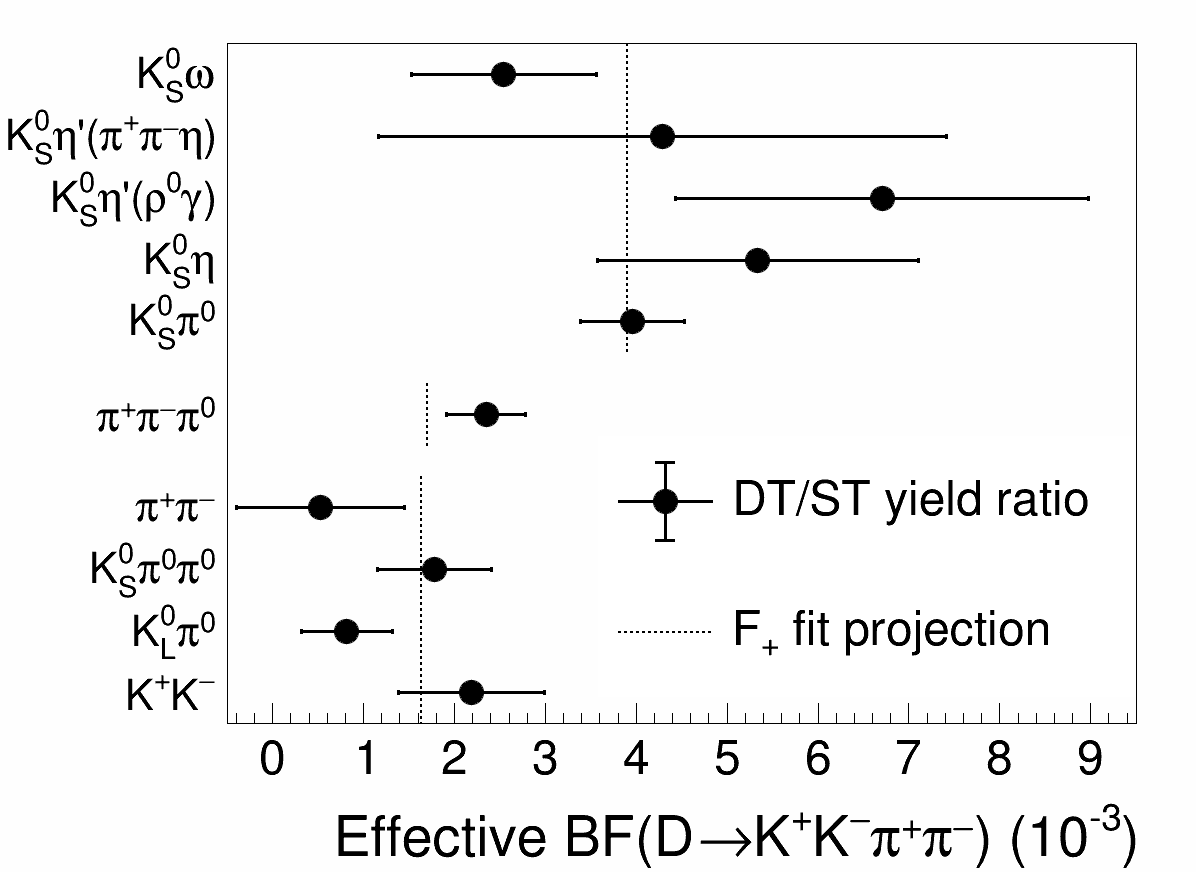
\includegraphics[width = 0.6\textwidth]{Plots/CPeven_fraction_combination_CPtags.png}
  \end{figure}
  \begin{equation*}
    \frac{N^{\rm DT}(KK\pi\pi | f)}{N^{\rm ST}(f)}\times\frac{\epsilon^{\rm ST}(f)}{\epsilon^{\rm DT}(KK\pi\pi | f)} = \mathcal{B}(KK\pi\pi)\Big(1 - (2F_+ - 1)(2F_+^f - 1)\Big)
  \end{equation*}
  \begin{center}
    Count ST and DT yields and fit, with $F_+$ and $\mathcal{B}(KK\pi\pi)$ as free parameters
  \end{center}
\end{frame}

\begin{frame}{Formalism for binned phase space measurement}
  \begin{center}
    Equation for binned analysis is analogous, but more complicated
  \end{center}
  \begin{align*}
    \frac{N_i^{\rm DT}(KK\pi\pi | f)}{N^{\rm ST}(f)}\times&\frac{\epsilon^{\rm ST}(f)}{\epsilon^{\rm DT}(KK\pi\pi | f)} =\\
    &\mathcal{B}(KK\pi\pi)\Big(K_i + K_{-i} - 2\sqrt{K_iK_{-i}}(2F_+^f - 1)c_i\Big)
  \end{align*}
  \vspace{-0.7cm}
  \begin{itemize}
    \item{$i$ labels the phase space bin}
    \item{$K_i$ is the fractional bin yield}
    \item{$c_i$ is the amplitude averaged cosine of the strong phase}
    \begin{itemize}
      \item{For a single bin, $c_i = 2F_+ - 1$}
    \end{itemize}
    \item{Binning scheme:}
    \begin{enumerate}
      \item{Preliminary studies with $\SI{3}{\per\femto\barn}$ dataset: $2\times2$ bins}
      \item{Analysis for thesis with $\SI{8}{\per\femto\barn}$ dataset: $2\times4$ bins}
      \item{Future analysis with $\SI{20}{\per\femto\barn}$ dataset: $2\times8$ bins}
    \end{enumerate}
  \end{itemize}
\end{frame}

\begin{frame}{Measurement of \texorpdfstring{$K_i$}{Ki}}
  \begin{figure}
    \centering
    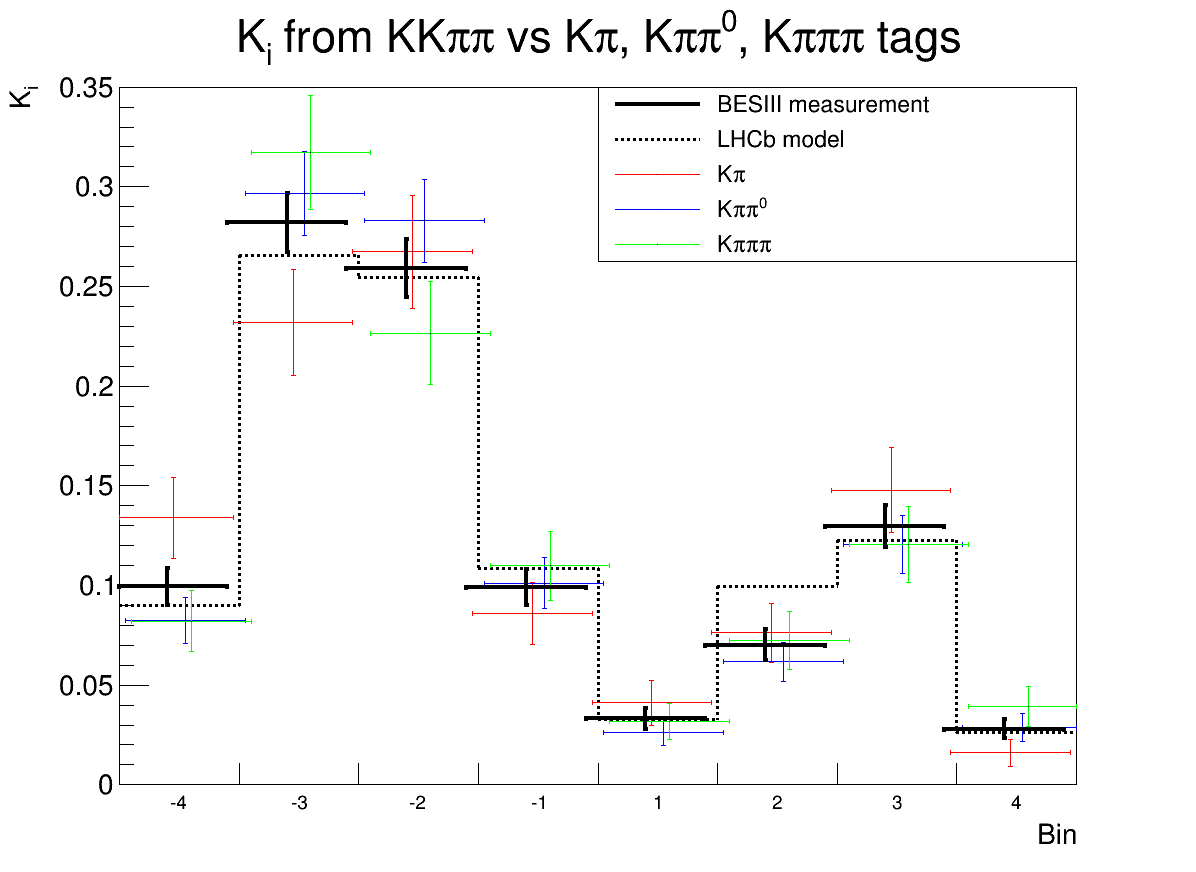
\includegraphics[width = 0.7\textwidth]{Plots/Ki_Measured_vs_Model_normalised.png}
  \end{figure}
  \vspace{-0.6cm}
  \begin{itemize}
    \item{Old plot shown in charm WG last year}
    \item{Cross check between BESIII data and LHCb model}
    \item{\underline{Normalised} bin yields show good bin-to-bin agreement}
  \end{itemize}
\end{frame}

\begin{frame}{Measurement of \texorpdfstring{$K_i$}{Ki}}
  \begin{figure}
    \centering
    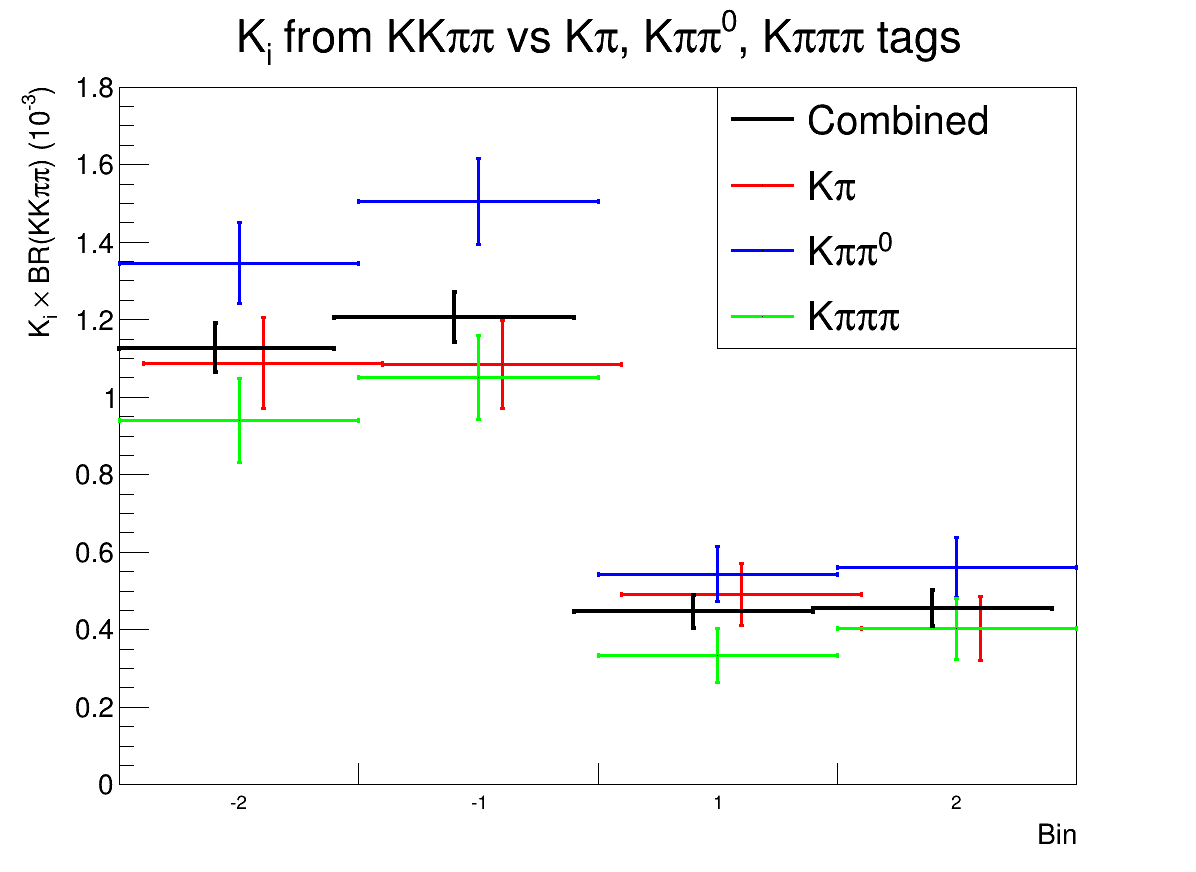
\includegraphics[width = 0.6\textwidth]{Plots/Ki_Measured_vs_Model.png}
  \end{figure}
  \vspace{-0.6cm}
  \begin{itemize}
    \item{Redone measurement with reduced $2\times2$ binning scheme}
    \item{This time, I'm looking at the absolute DT to ST yield}
    \item{$K_i$ from $K\pi\pi\pi^0$ yields are all larger than $K\pi$ and $K\pi\pi\pi$ tags -- systematic effect in $\pi^0$ modelling...?}
    \item{Not really an issue, just let $\mathcal{B}(KK\pi\pi)$ float in the fit}
  \end{itemize}
\end{frame}

\begin{frame}{Fit yield of some CP tags}
  \begin{center}
    Do simultaneous double tag yield fit of CP tags
  \end{center}
  \begin{figure}
    \centering
    \begin{subfigure}{0.49\textwidth}
      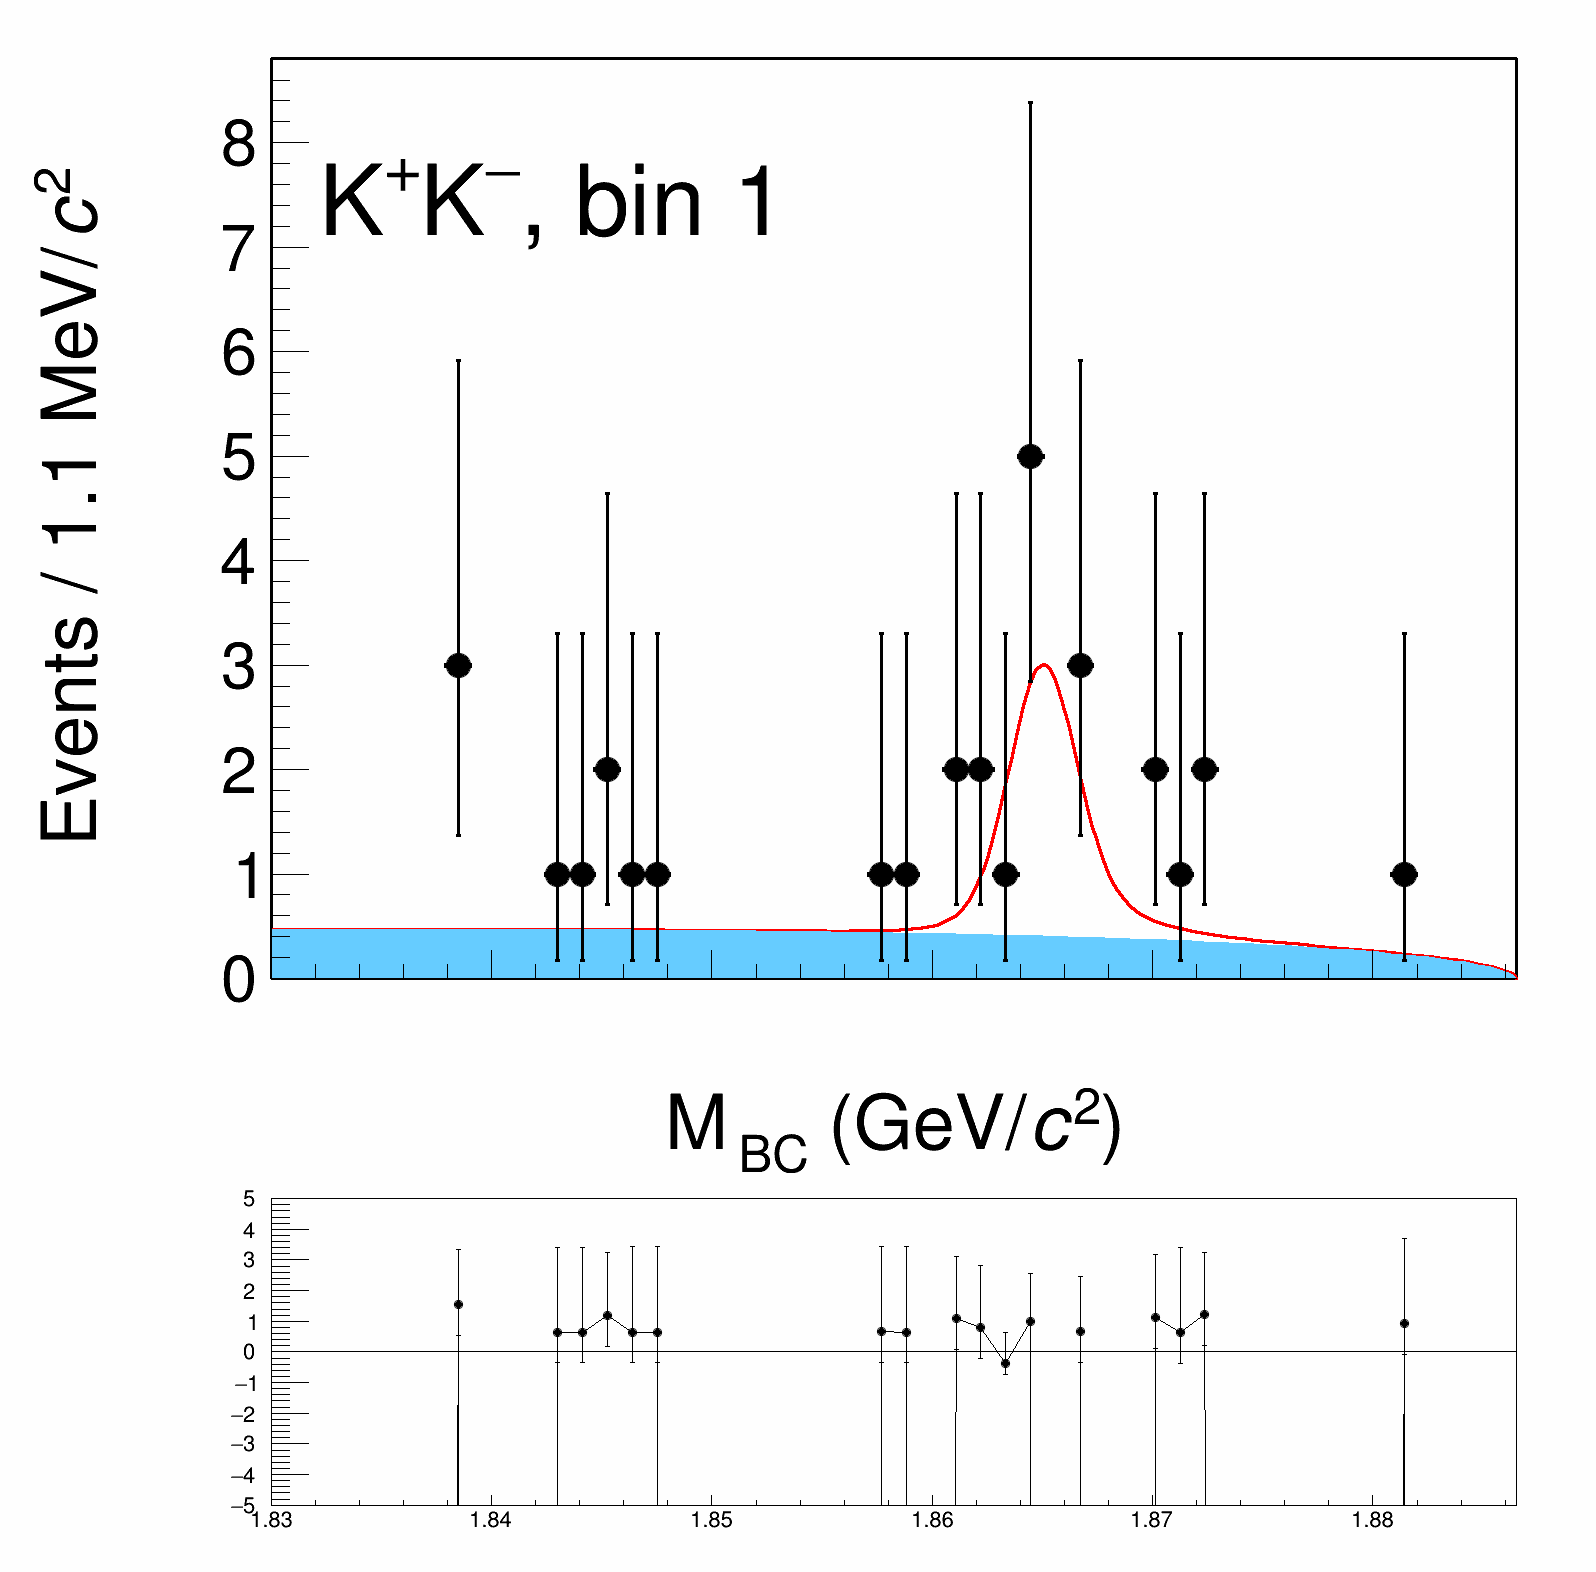
\includegraphics[width = 1.0\textwidth, trim = {0 14cm 0 0}, clip = true]{Plots/DoubleTagYield_DoubleTag_CP_KKpipi_vs_KK_SignalBin1.png}
      \caption{$10.2^{+6.7}_{-3.9}$}
    \end{subfigure}%
    \begin{subfigure}{0.49\textwidth}
      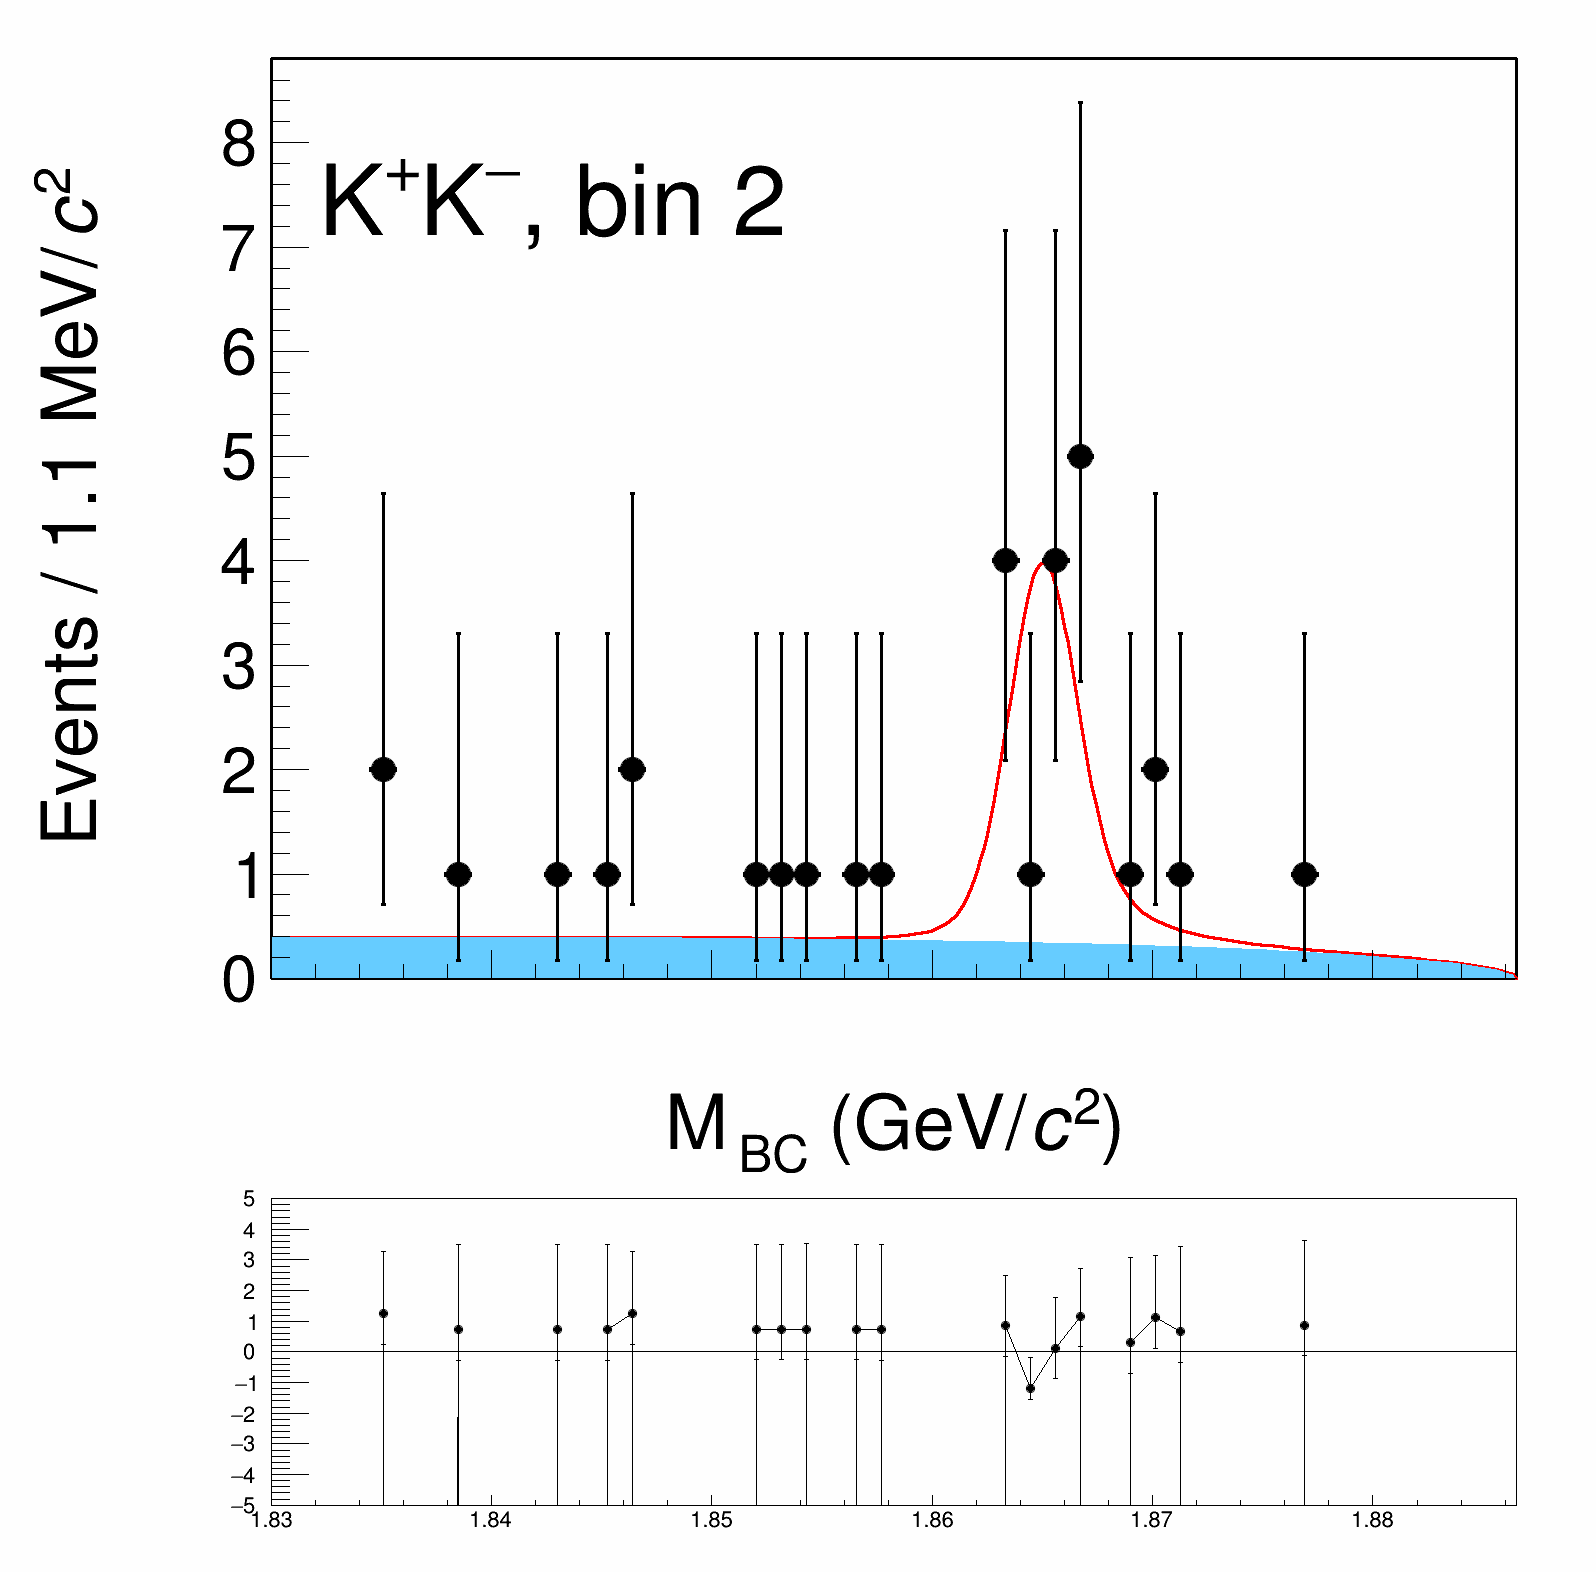
\includegraphics[width = 1.0\textwidth, trim = {0 14cm 0 0}, clip = true]{Plots/DoubleTagYield_DoubleTag_CP_KKpipi_vs_KK_SignalBin2.png}
      \caption{$14.4^{+4.8}_{-4.1}$}
    \end{subfigure}
    \caption{$KK\pi\pi$ vs $KK$}
  \end{figure}
\end{frame}

\begin{frame}{Fit yield of some CP tags}
  \begin{center}
    Do simultaneous double tag yield fit of CP tags
  \end{center}
  \begin{figure}
    \centering
    \begin{subfigure}{0.49\textwidth}
      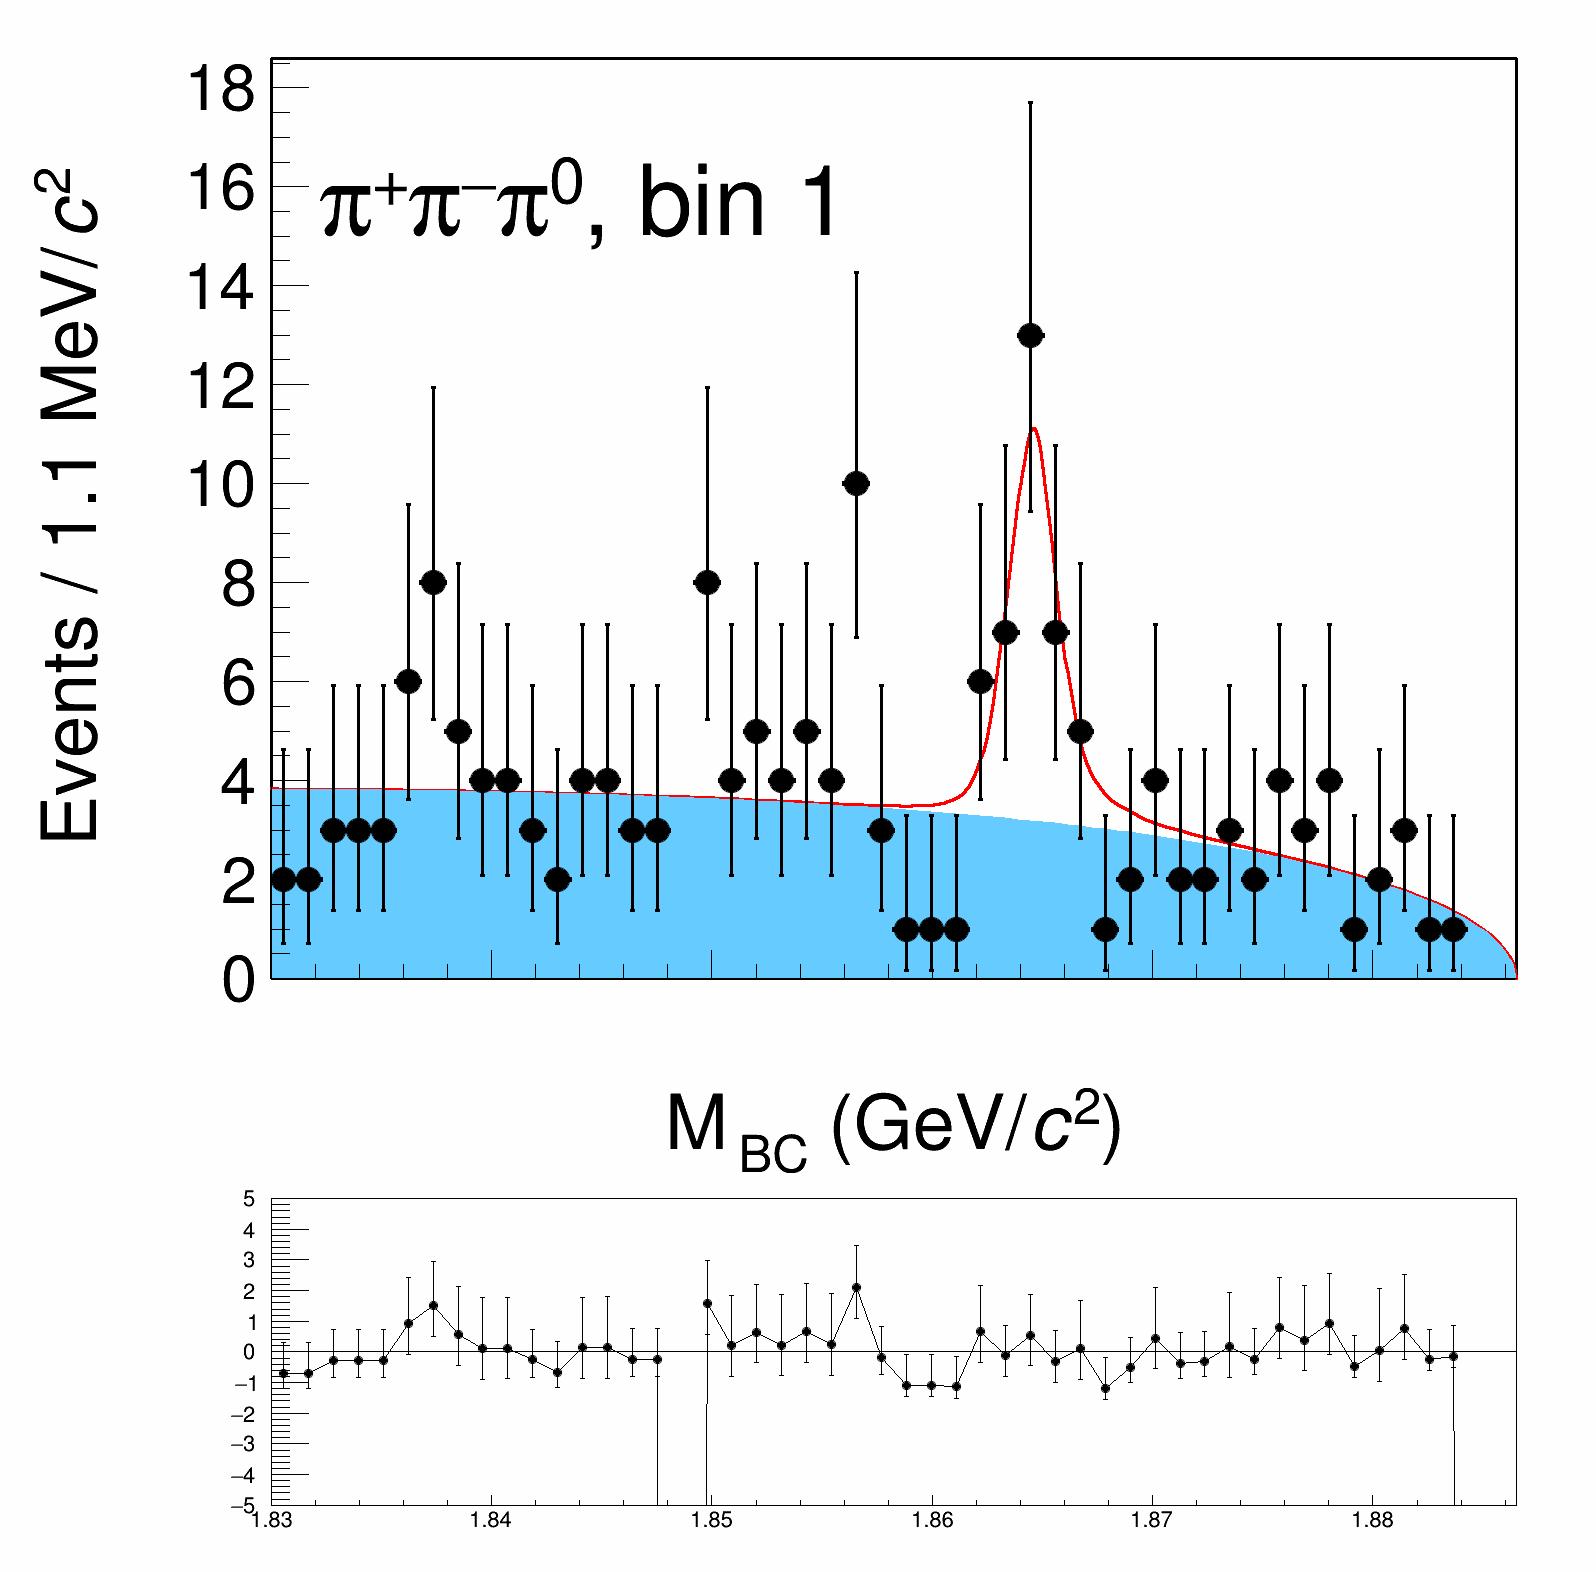
\includegraphics[width = 1.0\textwidth, trim = {0 14cm 0 0}, clip = true]{Plots/DoubleTagYield_DoubleTag_CP_KKpipi_vs_pipipi0_SignalBin1.png}
      \caption{$22.3^{+6.9}_{-6.2}$}
    \end{subfigure}%
    \begin{subfigure}{0.49\textwidth}
      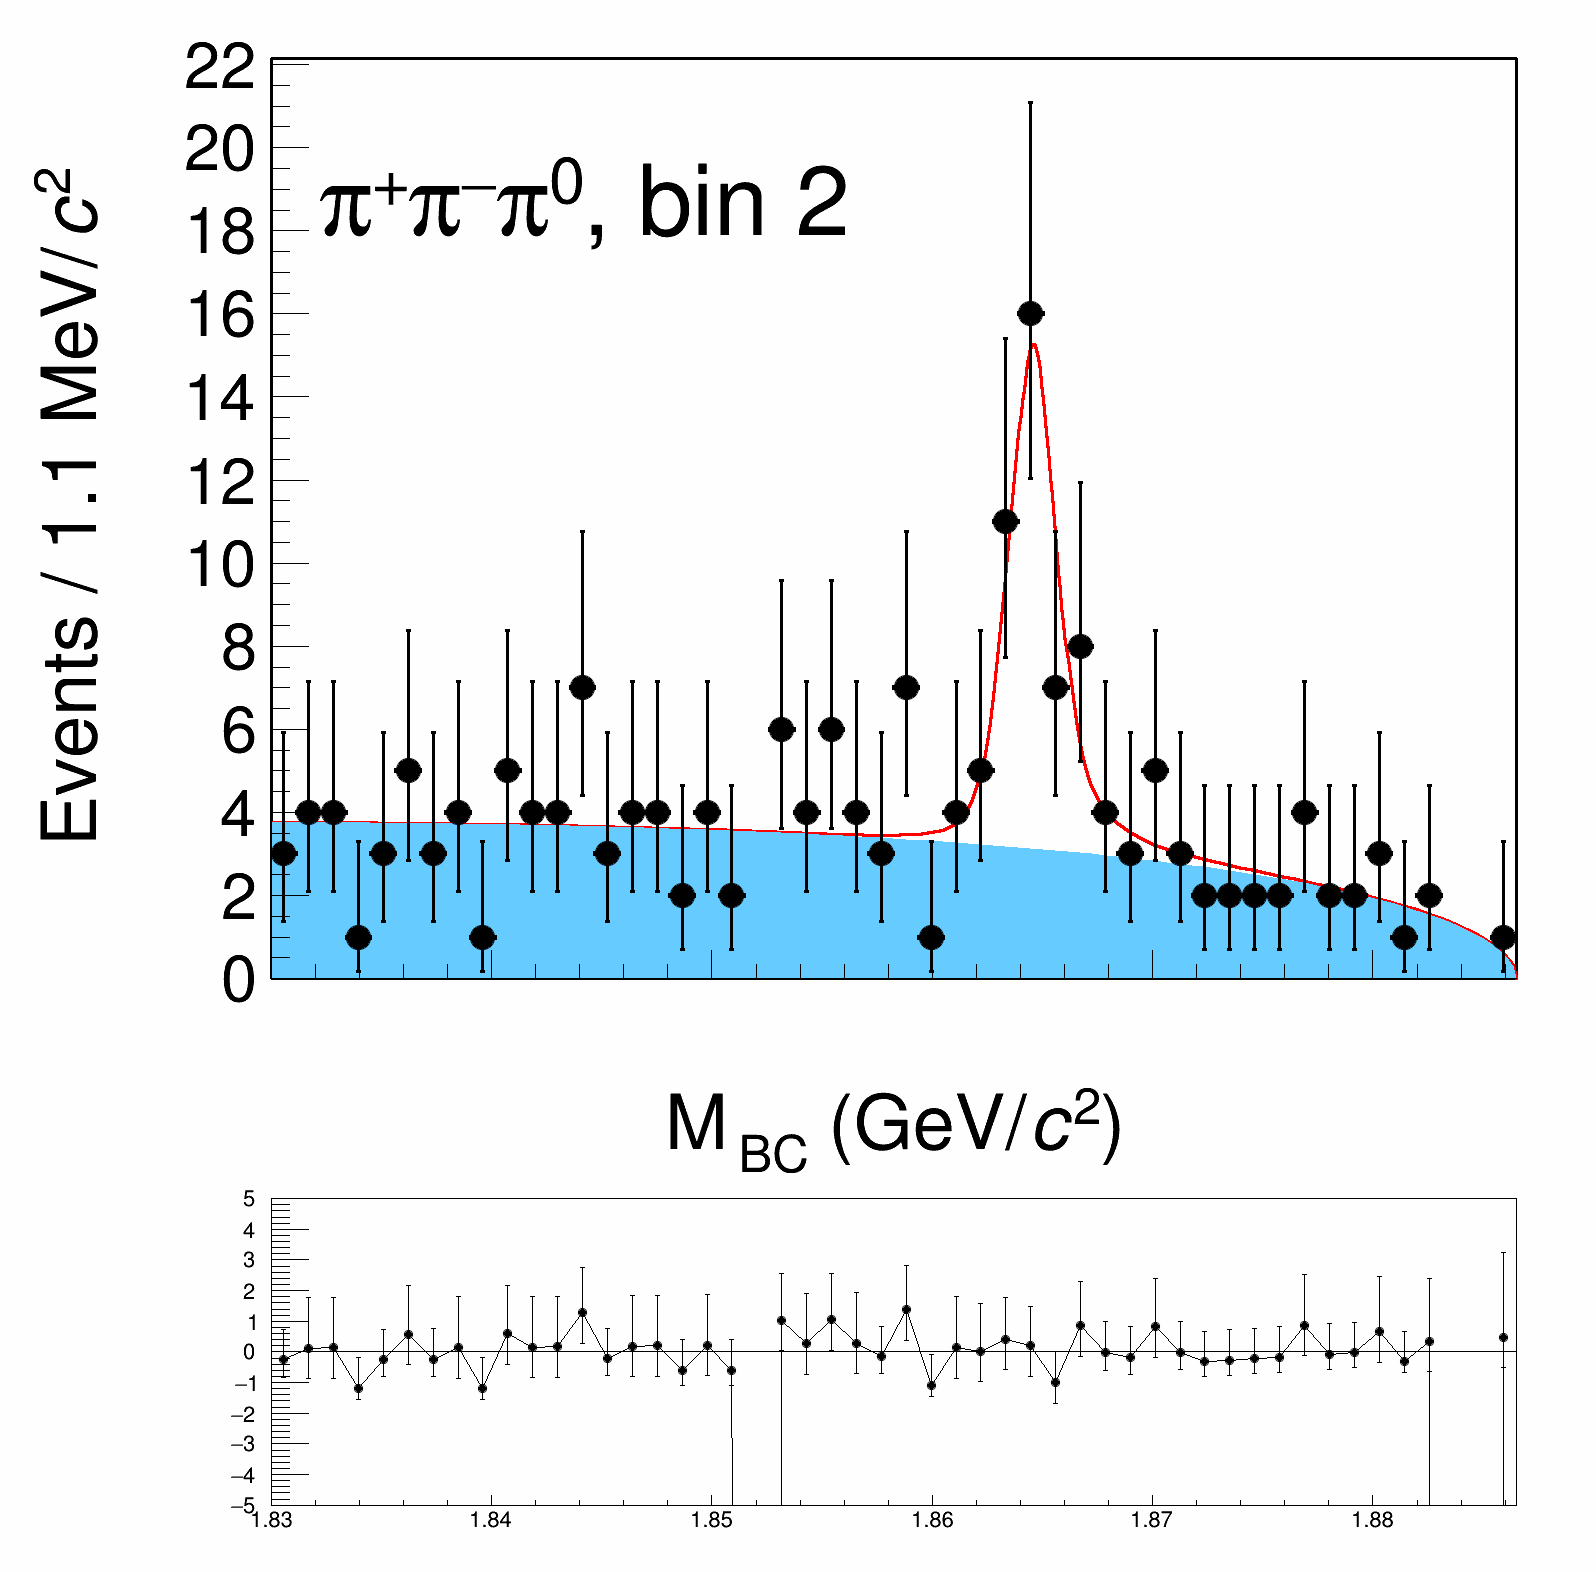
\includegraphics[width = 1.0\textwidth, trim = {0 14cm 0 0}, clip = true]{Plots/DoubleTagYield_DoubleTag_CP_KKpipi_vs_pipipi0_SignalBin2.png}
      \caption{$34.2^{+8.0}_{-7.3}$}
    \end{subfigure}
    \caption{$KK\pi\pi$ vs $\pi\pi\pi^0$}
  \end{figure}
\end{frame}

\begin{frame}{Fit yield of some CP tags}
  \begin{center}
    Do simultaneous double tag yield fit of CP tags
  \end{center}
  \begin{figure}
    \centering
    \begin{subfigure}{0.49\textwidth}
      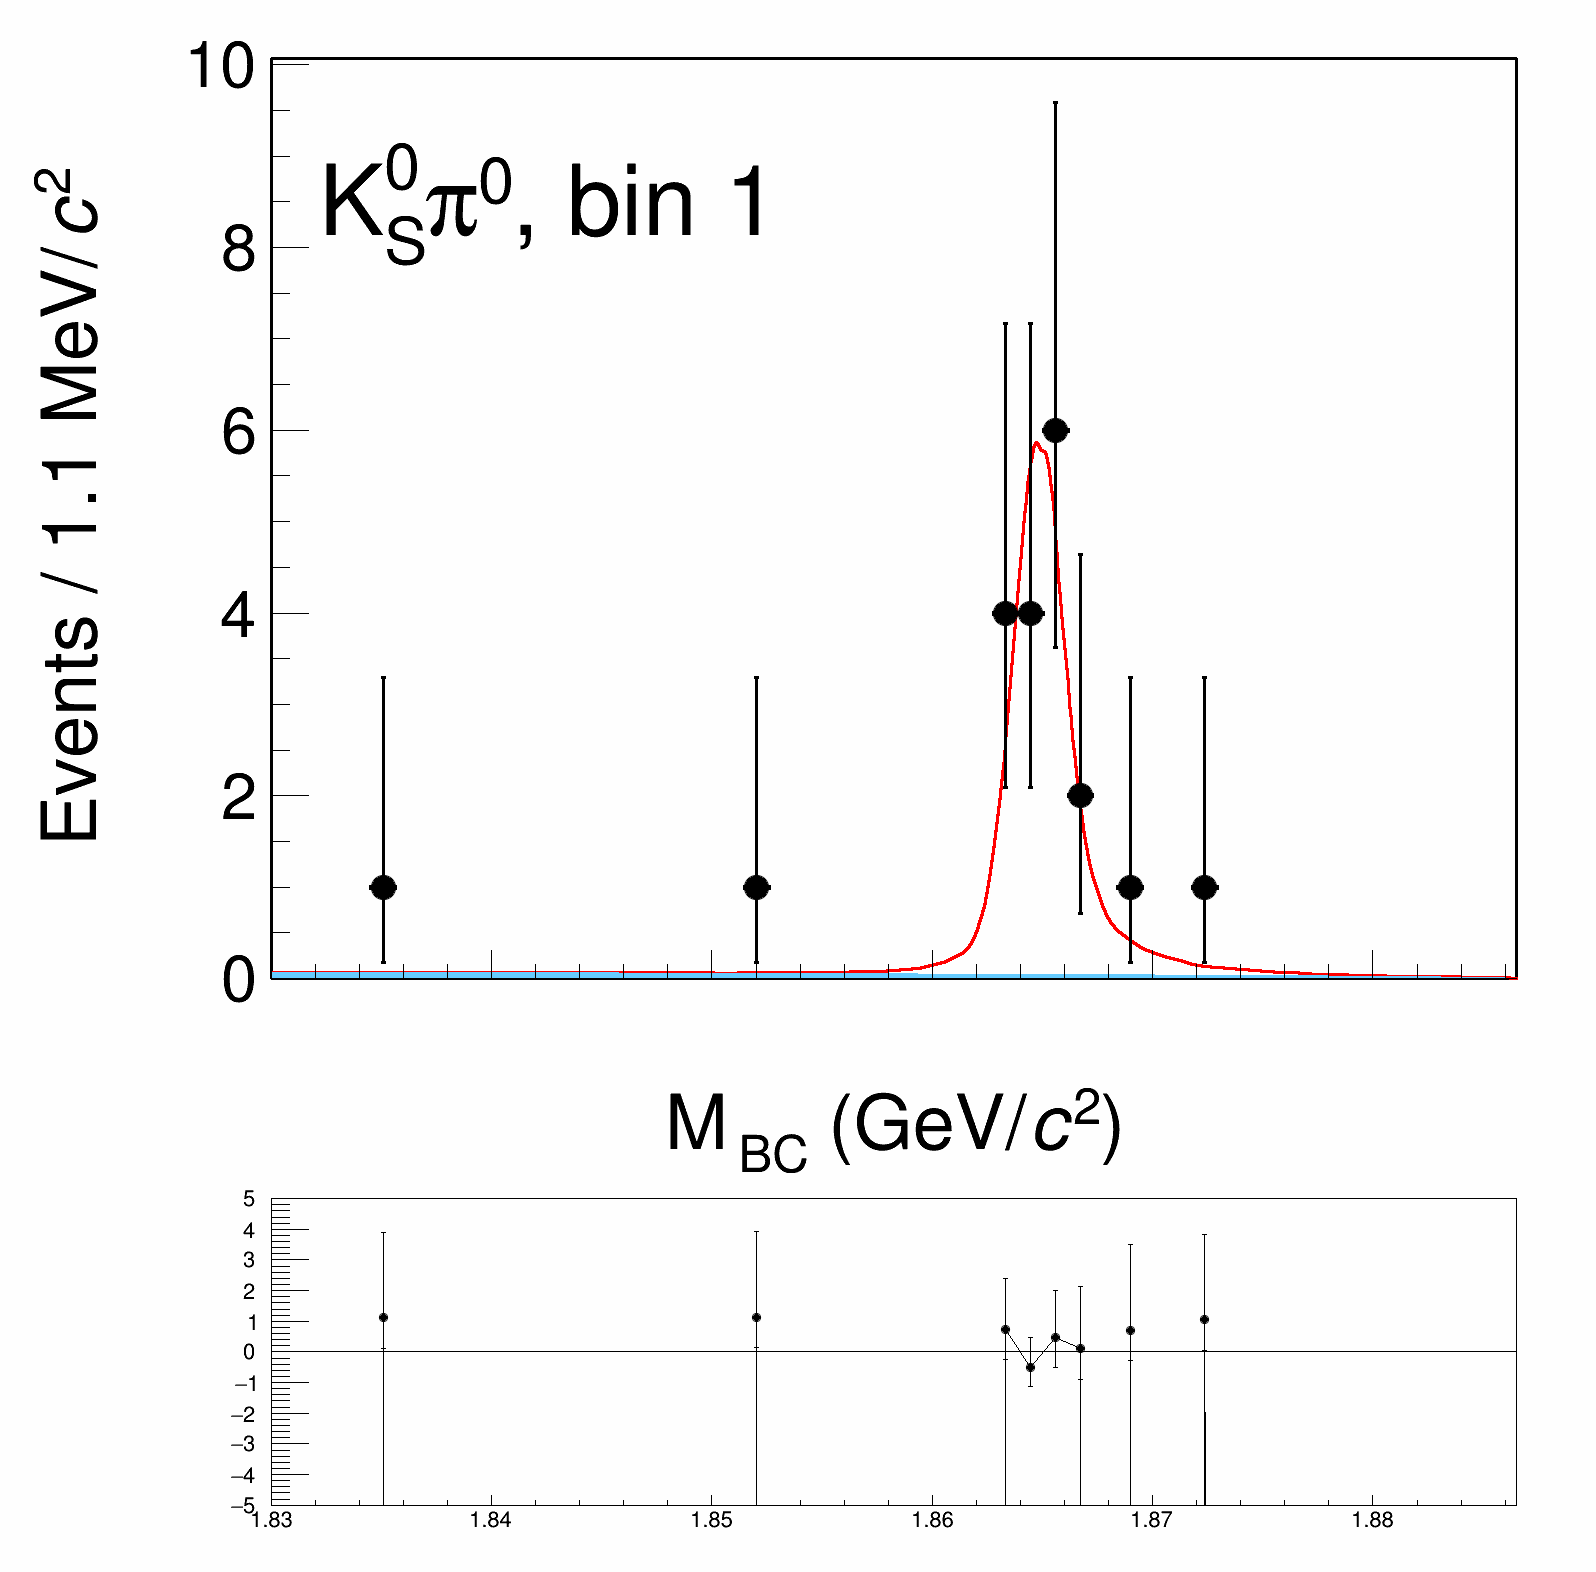
\includegraphics[width = 1.0\textwidth, trim = {0 14cm 0 0}, clip = true]{Plots/DoubleTagYield_DoubleTag_CP_KKpipi_vs_KSpi0_SignalBin1.png}
    \caption{$17.6^{+4.6}_{-3.9}$}
    \end{subfigure}%
    \begin{subfigure}{0.49\textwidth}
      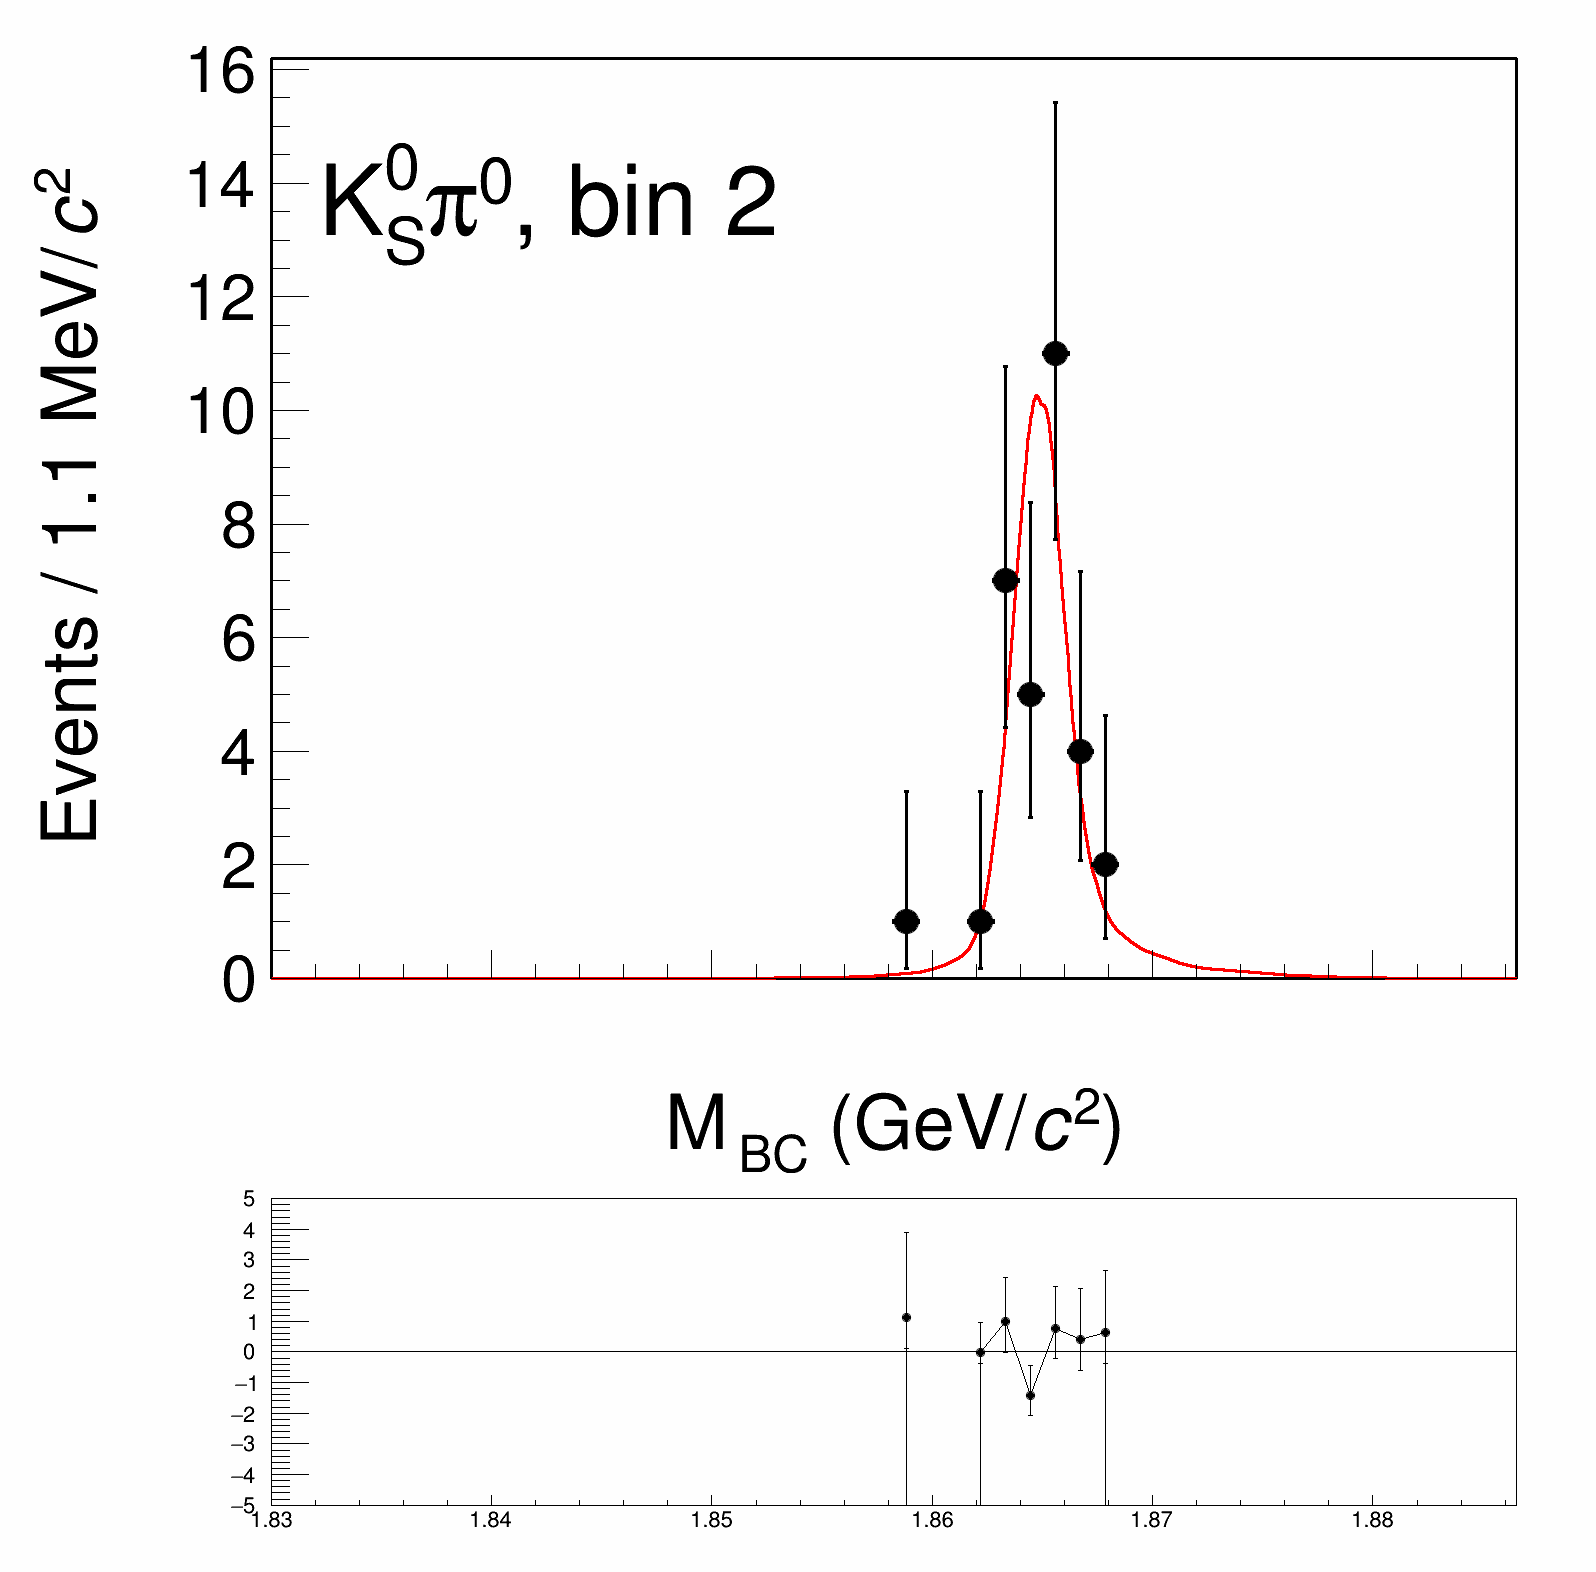
\includegraphics[width = 1.0\textwidth, trim = {0 14cm 0 0}, clip = true]{Plots/DoubleTagYield_DoubleTag_CP_KKpipi_vs_KSpi0_SignalBin2.png}
      \caption{$31.0^{+5.9}_{-5.2}$}
    \end{subfigure}
    \caption{$KK\pi\pi$ vs $K_S\pi^0$}
  \end{figure}
\end{frame}

\begin{frame}{Maximum likelihood fit of \texorpdfstring{$c_i$}{ci}}
  \begin{center}
    I have also worked on the maximum likelihood fit of $c_i$ (and $s_i$)
  \end{center}
  \begin{align*}
    \mathcal{L} =& [V^{-1}]_{ij}(N_i - \hat{N}_i)(N_j - \hat{N}_j) \\
    V_{ij} =& \rho_{ij}\sigma_i(N_i - \hat{N}_i)\sigma_j(N_j - \hat{N}_j) \\
    \sigma(N - \hat{N}) =& \sqrt{\sigma_+\sigma_- + (\sigma_+ - \sigma_-)(N - \hat{N})}
  \end{align*}
  \begin{itemize}
    \setlength\itemsep{1.0em}
    \item{$N$ are the double tag yields measured in data}
    \item{$\hat{N}$ are the predicted double tag yields from the value of $c_i$ (and $s_i$)}
    \item{The linear extrapolation of the covariance $V$ is ideal for this analysis because of the asymmetric uncertainties in bins with low yields}
  \end{itemize}
\end{frame}

\begin{frame}{Let's do some toys!}
  \begin{center}
    Pulls for fit with $KK$, $\pi\pi\pi^0$ and $K_S\pi^0$ tags
  \end{center}
  \begin{figure}
    \centering
    \begin{subfigure}{0.49\textwidth}
      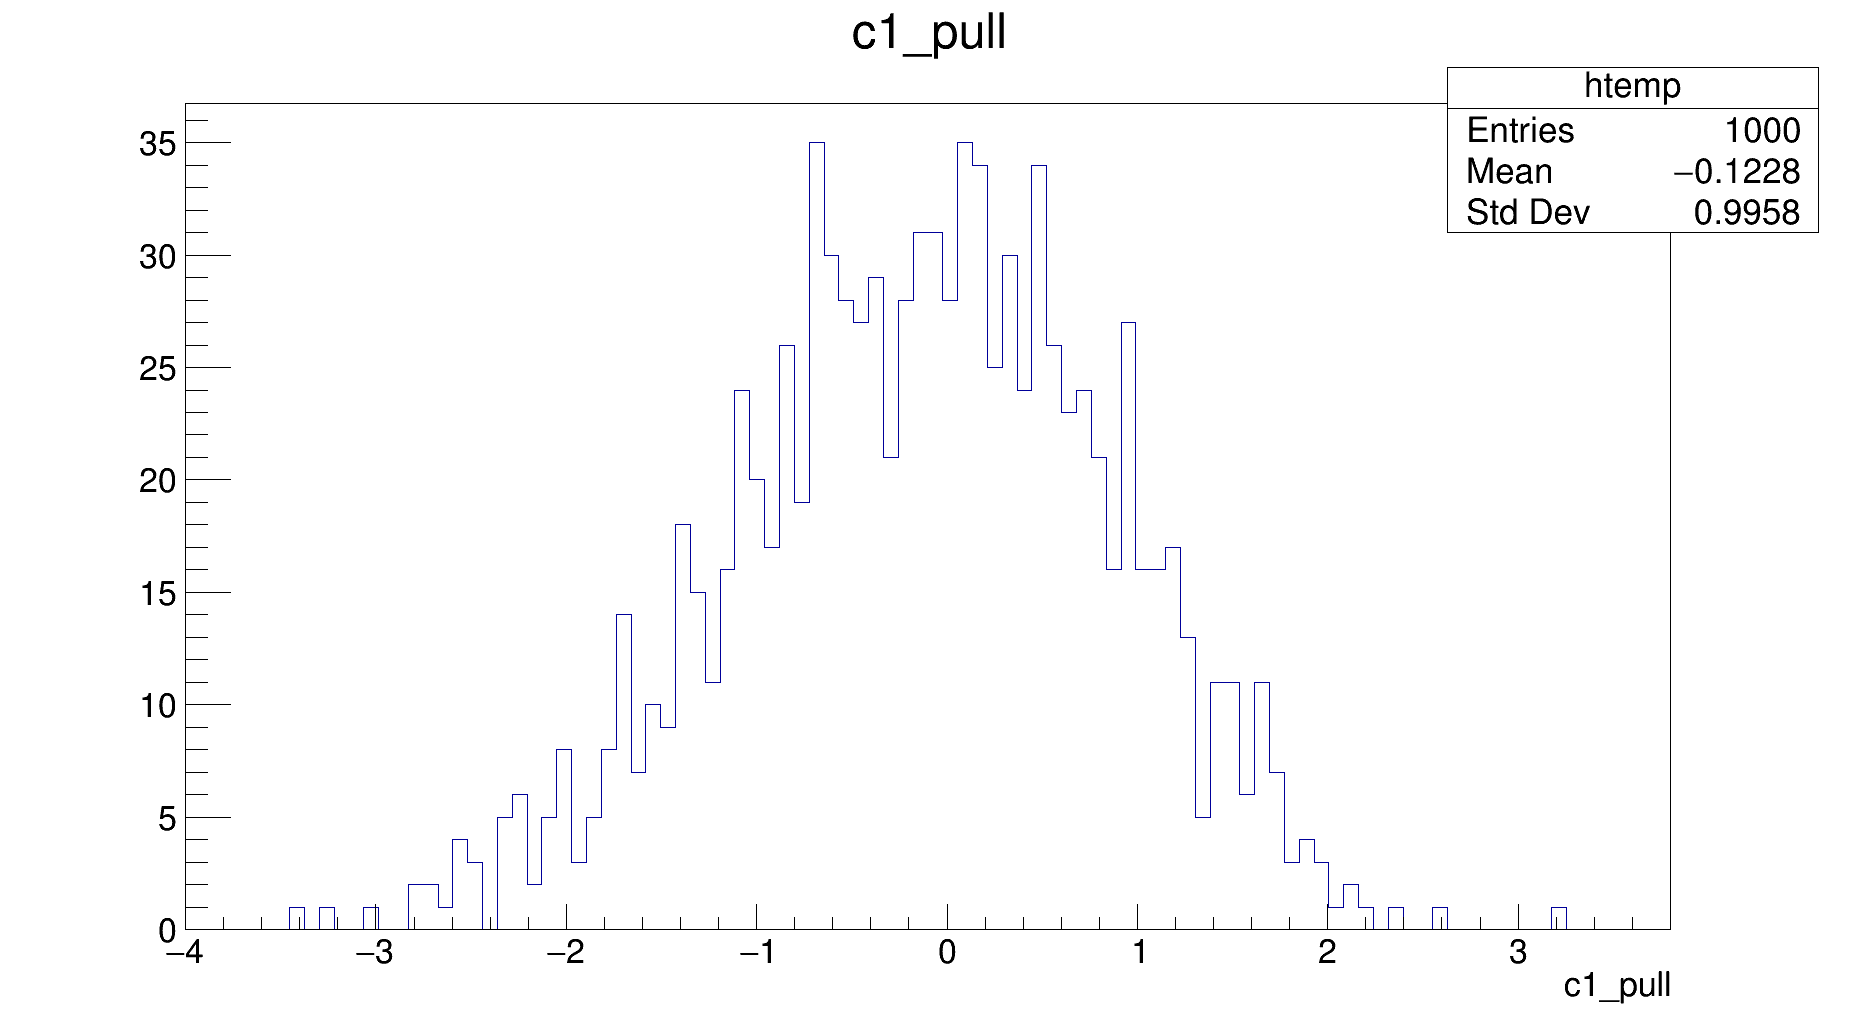
\includegraphics[width = 1.0\textwidth]{Plots/c1_pull.png}
    \end{subfigure}%
    \begin{subfigure}{0.49\textwidth}
      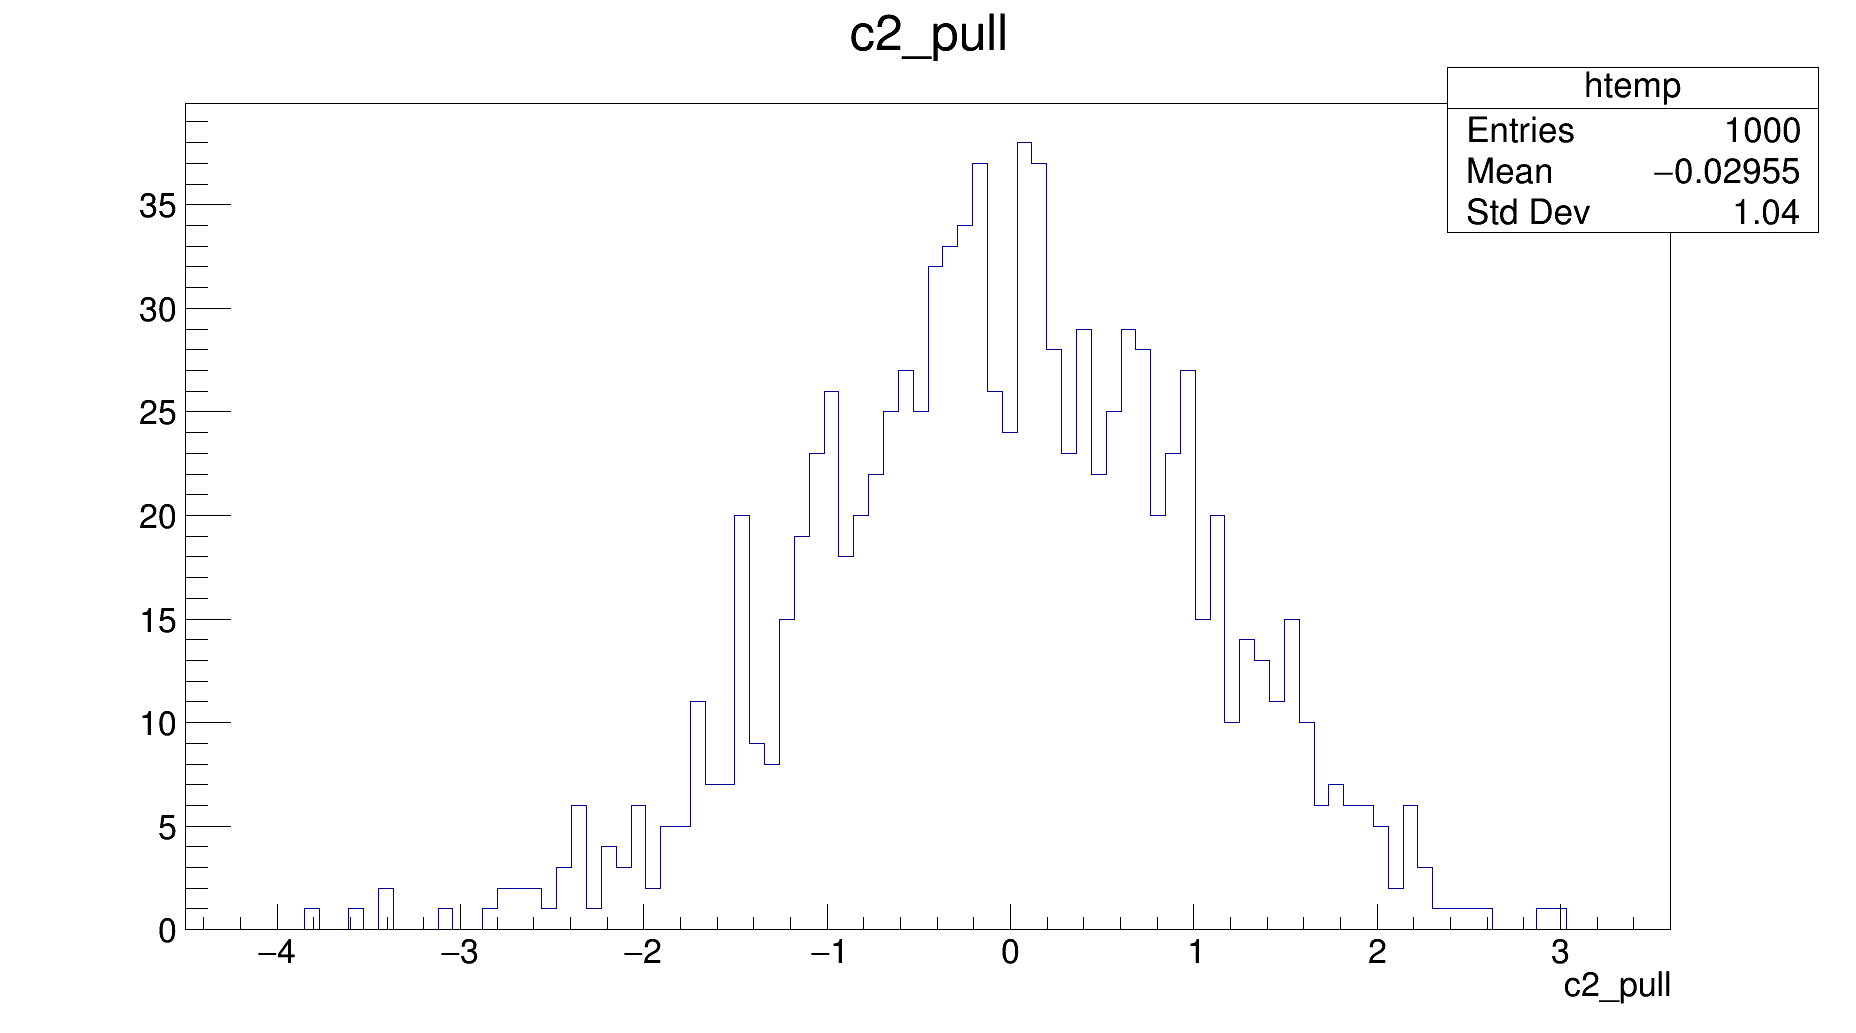
\includegraphics[width = 1.0\textwidth]{Plots/c2_pull.png}
    \end{subfigure}
  \end{figure}
  \begin{center}
    Bias in $c_1$ is likely because of low statistics, no bias seen in $c_2$
  \end{center}
\end{frame}

\begin{frame}{Let's do some toys!}
  \begin{figure}
    \centering
    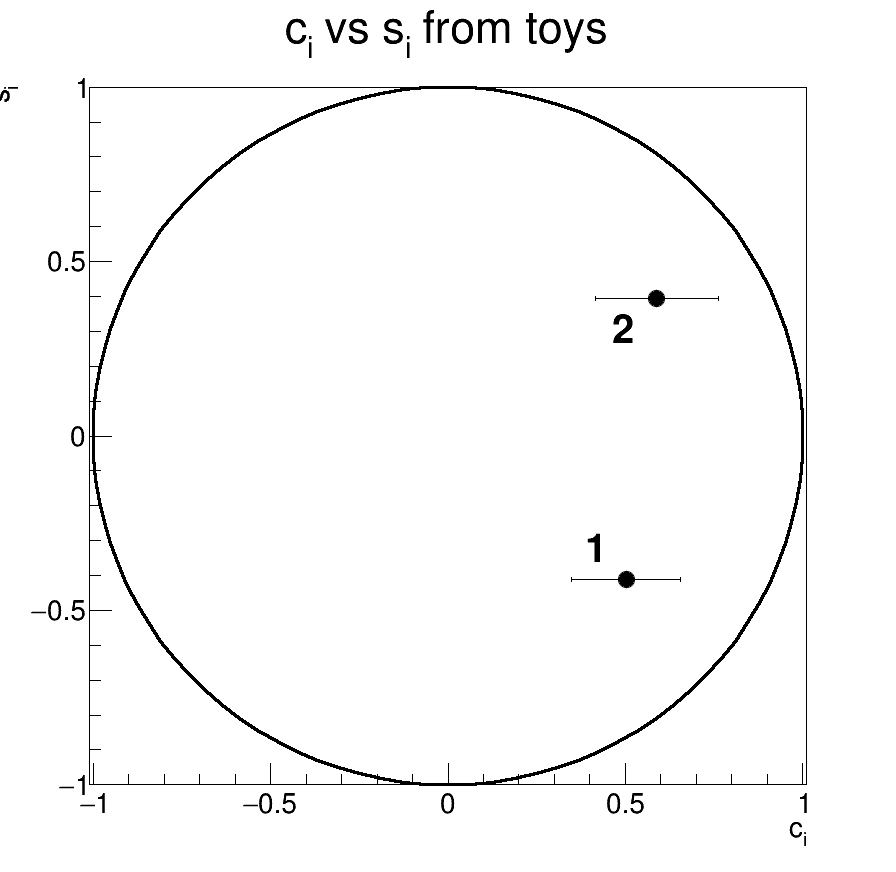
\includegraphics[width = 0.5\textwidth]{Plots/cisi_toys.png}
  \end{figure}
  \begin{itemize}
    \item{Expect these uncertainties to improve with the full $\SI{8}{\per\femto\barn}$ dataset}
    \item{Will also improve with additional fully and partially reconstructed $KK\pi\pi$ vs CP tags}
    \item{Should be sufficient statistics to do a fit with $2\times4$ bins}
  \end{itemize}
\end{frame}

\section{TORCH November 2022 testbeam}

\begin{frame}{TORCH November 2022 testbeam overview}
  \begin{figure}
    \centering
    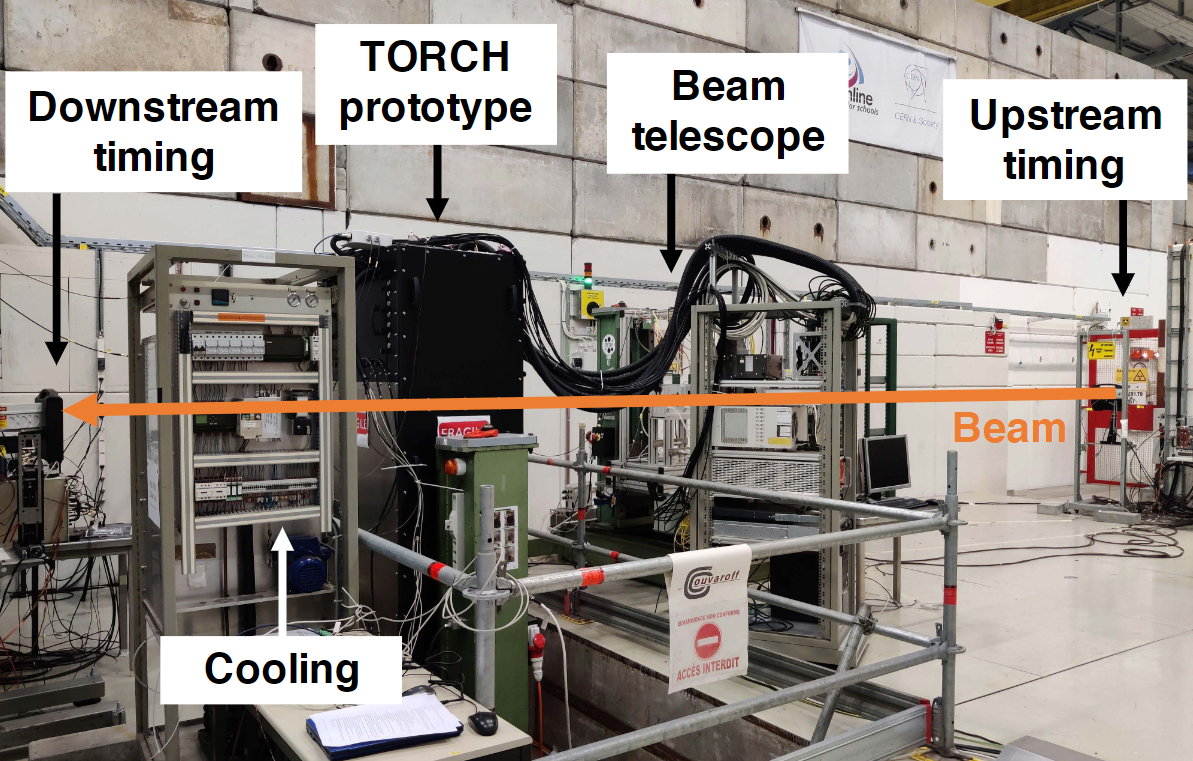
\includegraphics[width = 0.8\textwidth]{Plots/TORCH_overview.png}
    \caption{From Jenny's presentation 5th December}
  \end{figure}
  \vspace{-0.5cm}
  \begin{center}
    31st October -- 28th November 2022 at T9 PS Testbeam zone
  \end{center}
\end{frame}

\begin{frame}{Brief description of setup}
  \begin{center}
    \large
    TORCH testbeam relies on the following components:
  \end{center}
  \begin{enumerate}
    \setlength\itemsep{0.9em}
    \item{Beam information -- provided by the beam physicists at T9}
    \begin{itemize}
      \item{Large scintillators S0 and S1 to detect beam}
      \item{Cherenkov counters C0 and C1 to separate pions and protons}
    \end{itemize}
    \item{TORCH -- measure timing and Cherenkov angle of emitted photons}
    \item{Trigger -- take data when a track hits TORCH}
    \begin{itemize}
      \item{Small crossed scintillators at each timing station}
    \end{itemize}
    \item{Timing stations -- measure $T_0$ of the incident track}
    \begin{itemize}
      \item{Borosilicate fingers called F1 and F2}
    \end{itemize}
    \item{Beam telescope -- measure track incident position (won't cover this)}
    \item{Cooling -- should be obvious (won't cover this)}
  \end{enumerate}
\end{frame}

\begin{frame}{Week 1: Timing with (ancient) NIM modules}
  \begin{figure}
    \centering
    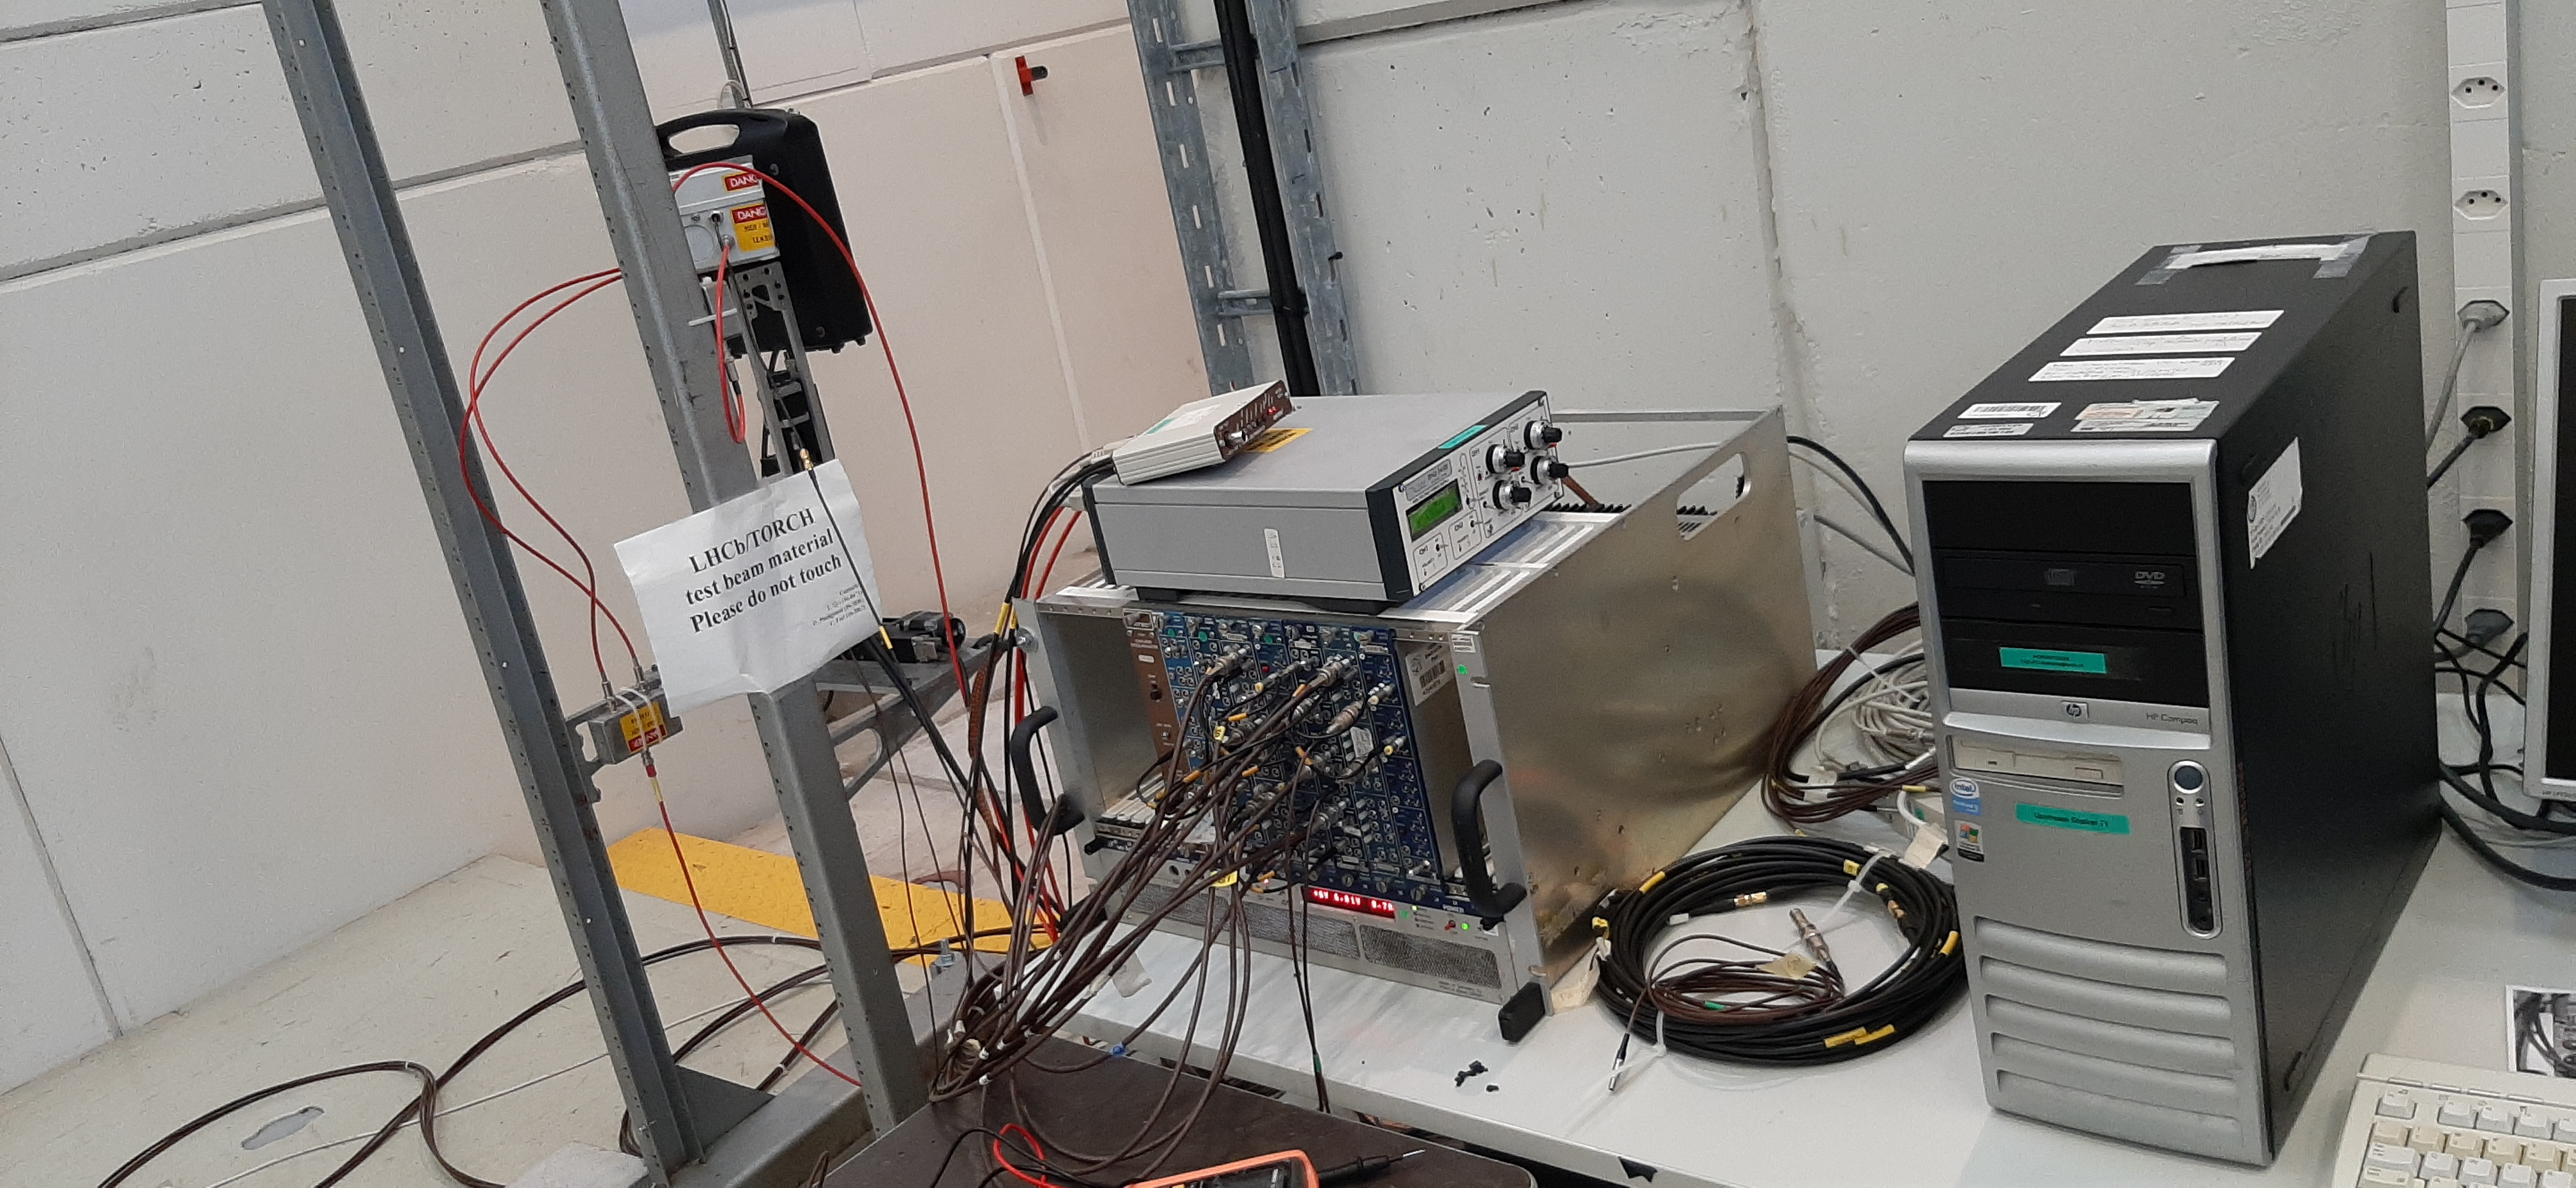
\includegraphics[width = 1.0\textwidth]{Plots/T1_overview.jpg}
    \caption{Timing station T1 (upstream) overview}
  \end{figure}
\end{frame}

\begin{frame}{Week 1: Timing with (ancient) NIM modules}
  \begin{figure}
    \centering
    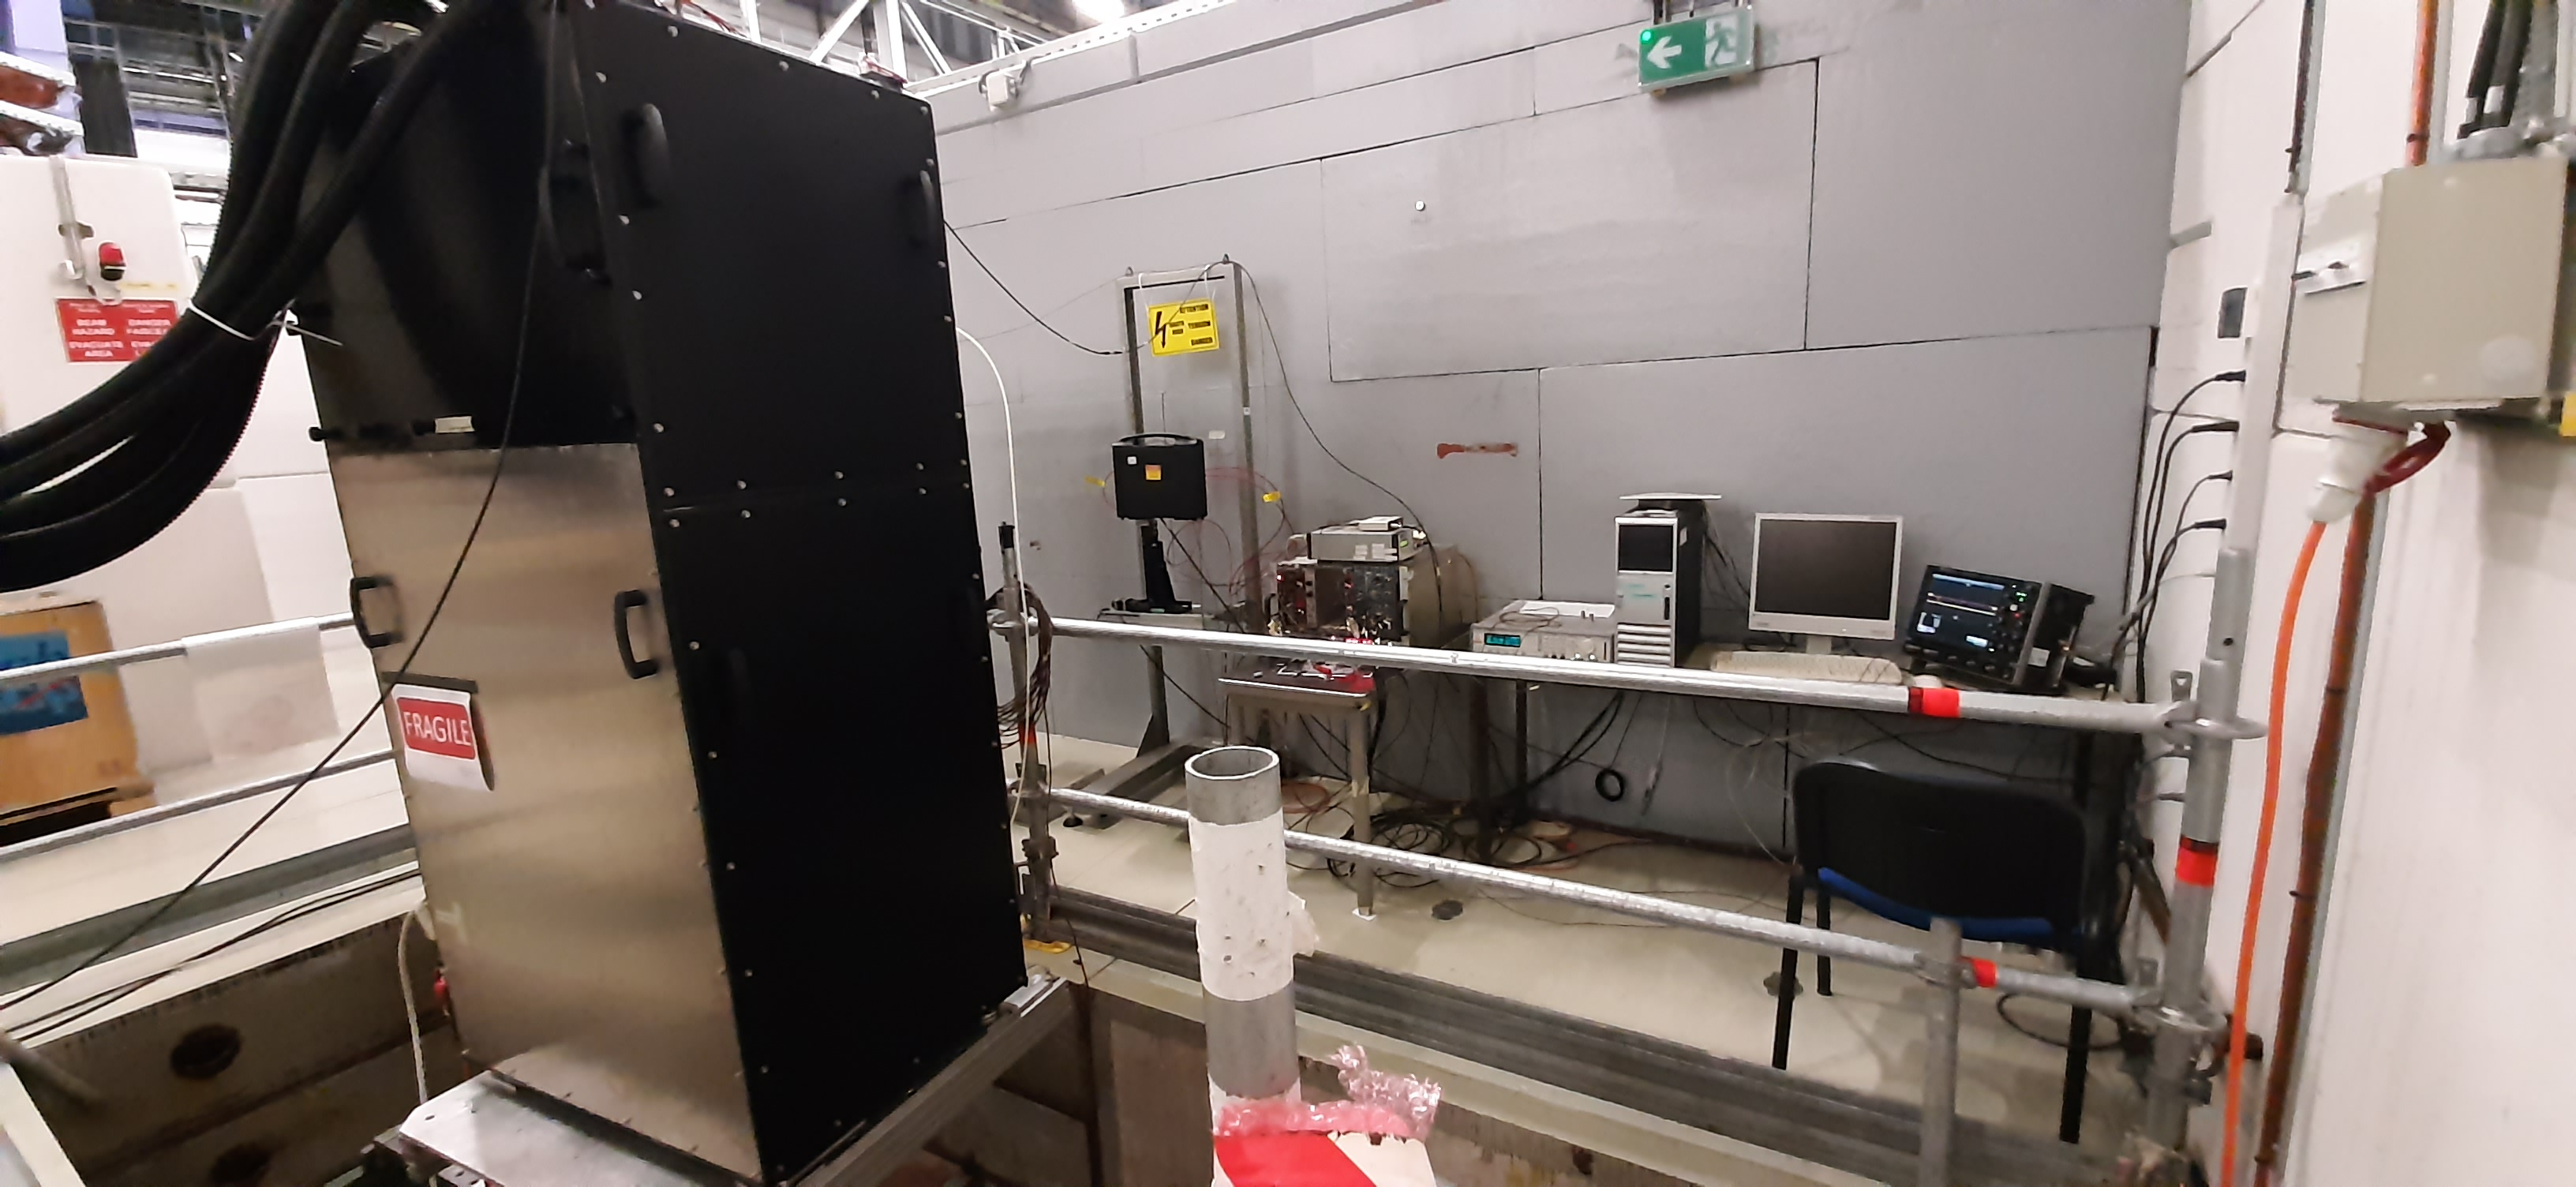
\includegraphics[width = 1.0\textwidth]{Plots/T2_overview.jpg}
    \caption{Timing station T2 (downstream) overview}
  \end{figure}
\end{frame}

\begin{frame}{Week 1: Timing with (ancient) NIM modules}
  \begin{figure}
    \centering
    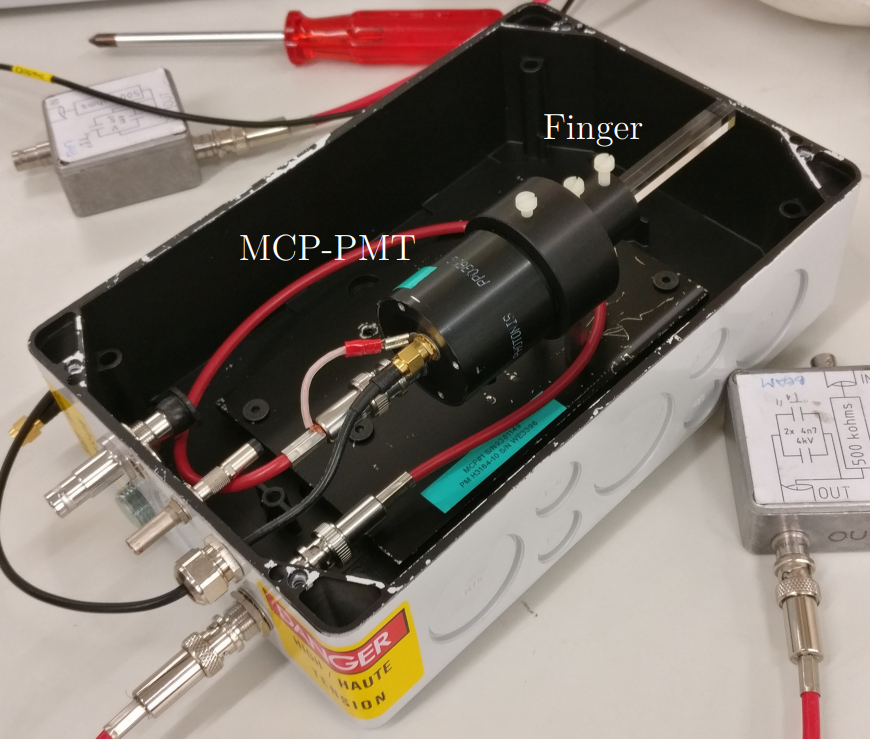
\includegraphics[width = 0.6\textwidth]{Plots/BorosilicateFinger.png}
    \caption{From Thomas Hancock's PhD thesis}
  \end{figure}
\end{frame}

\begin{frame}{Week 1: Timing with (ancient) NIM modules}
  \begin{figure}
    \centering
    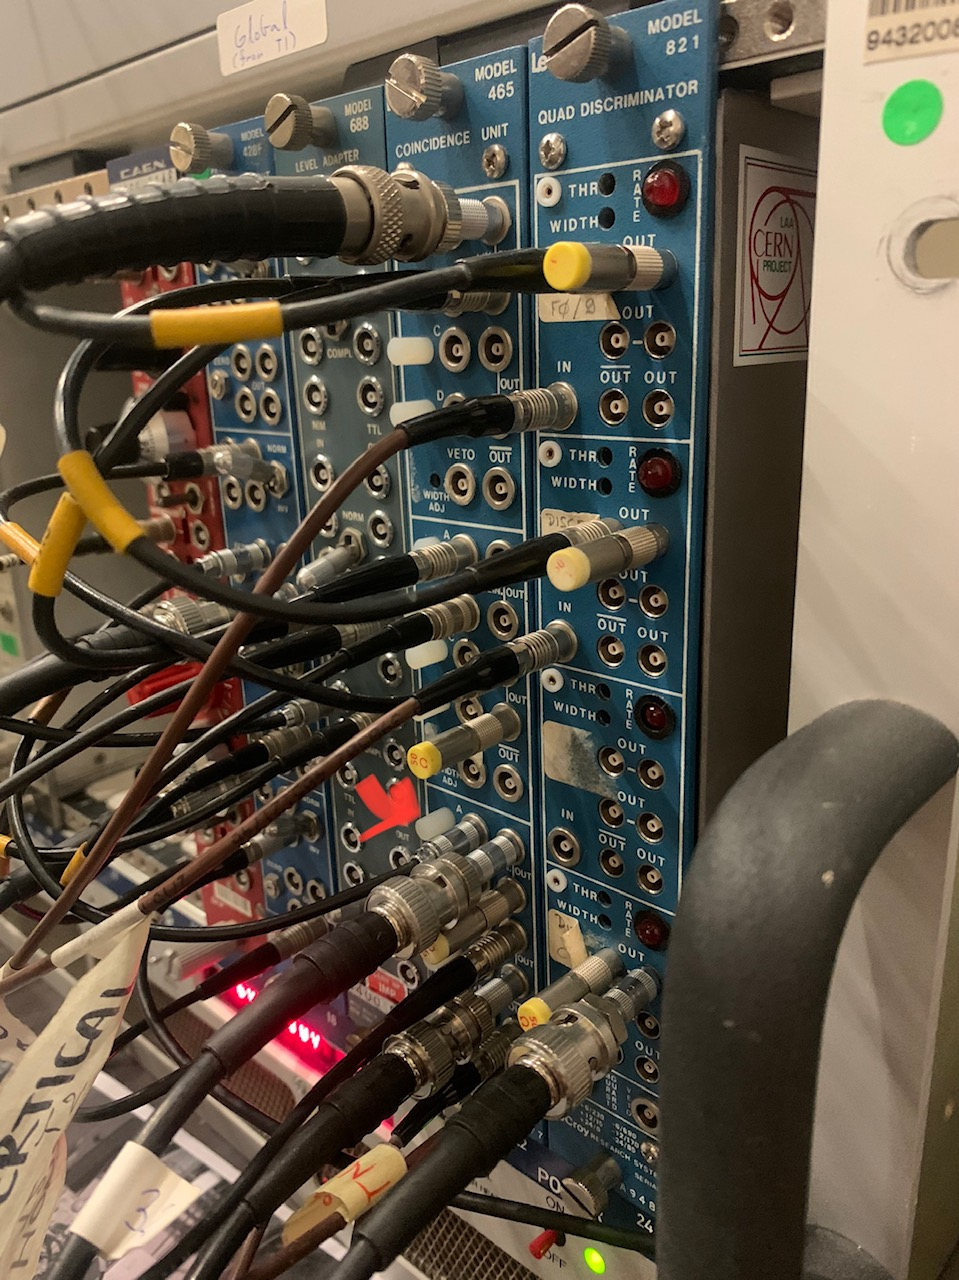
\includegraphics[width = 0.45\textwidth]{Plots/Cabling.jpg}
    \caption{Messy cabling}
  \end{figure}
\end{frame}

\begin{frame}{Week 1: Timing with (ancient) NIM modules}
  \begin{figure}
    \centering
    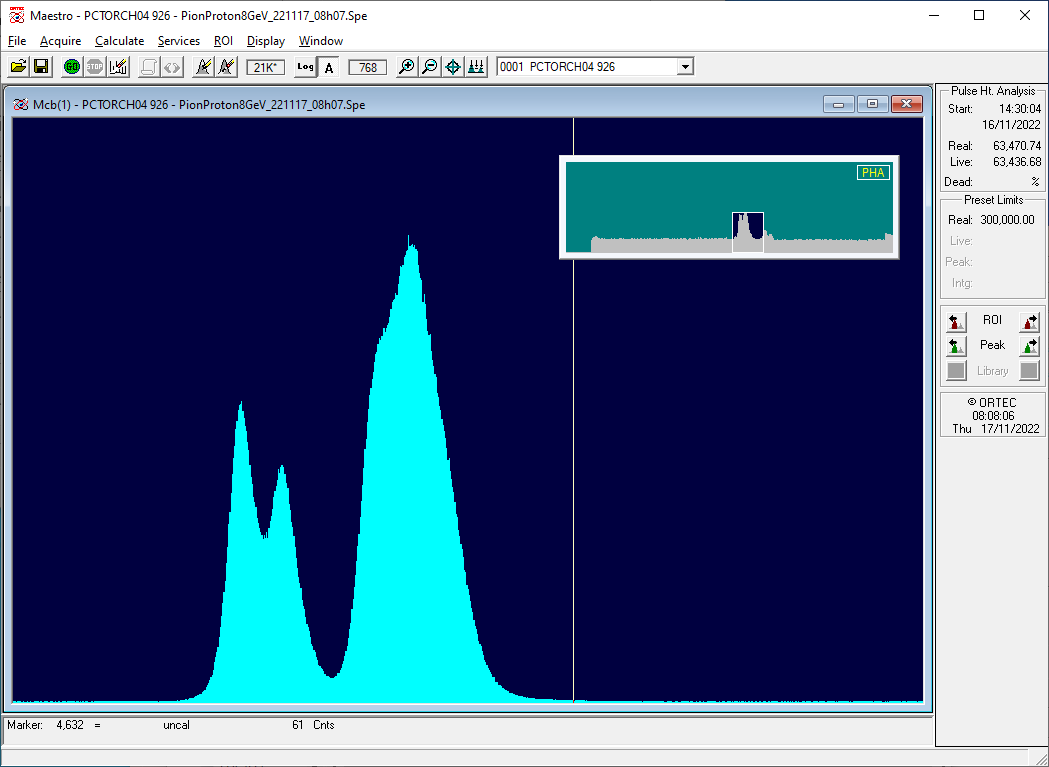
\includegraphics[width = 0.8\textwidth]{Plots/PionProton8GeV_221117_08h07.png}
    \caption{Timing histogram from F1 and F2, with a $\SI{6.3}{\pico\second}$ bin size}
  \end{figure}
\end{frame}

\begin{frame}{Week 2: TORCH arrives the zone}
  \begin{figure}
    \centering
    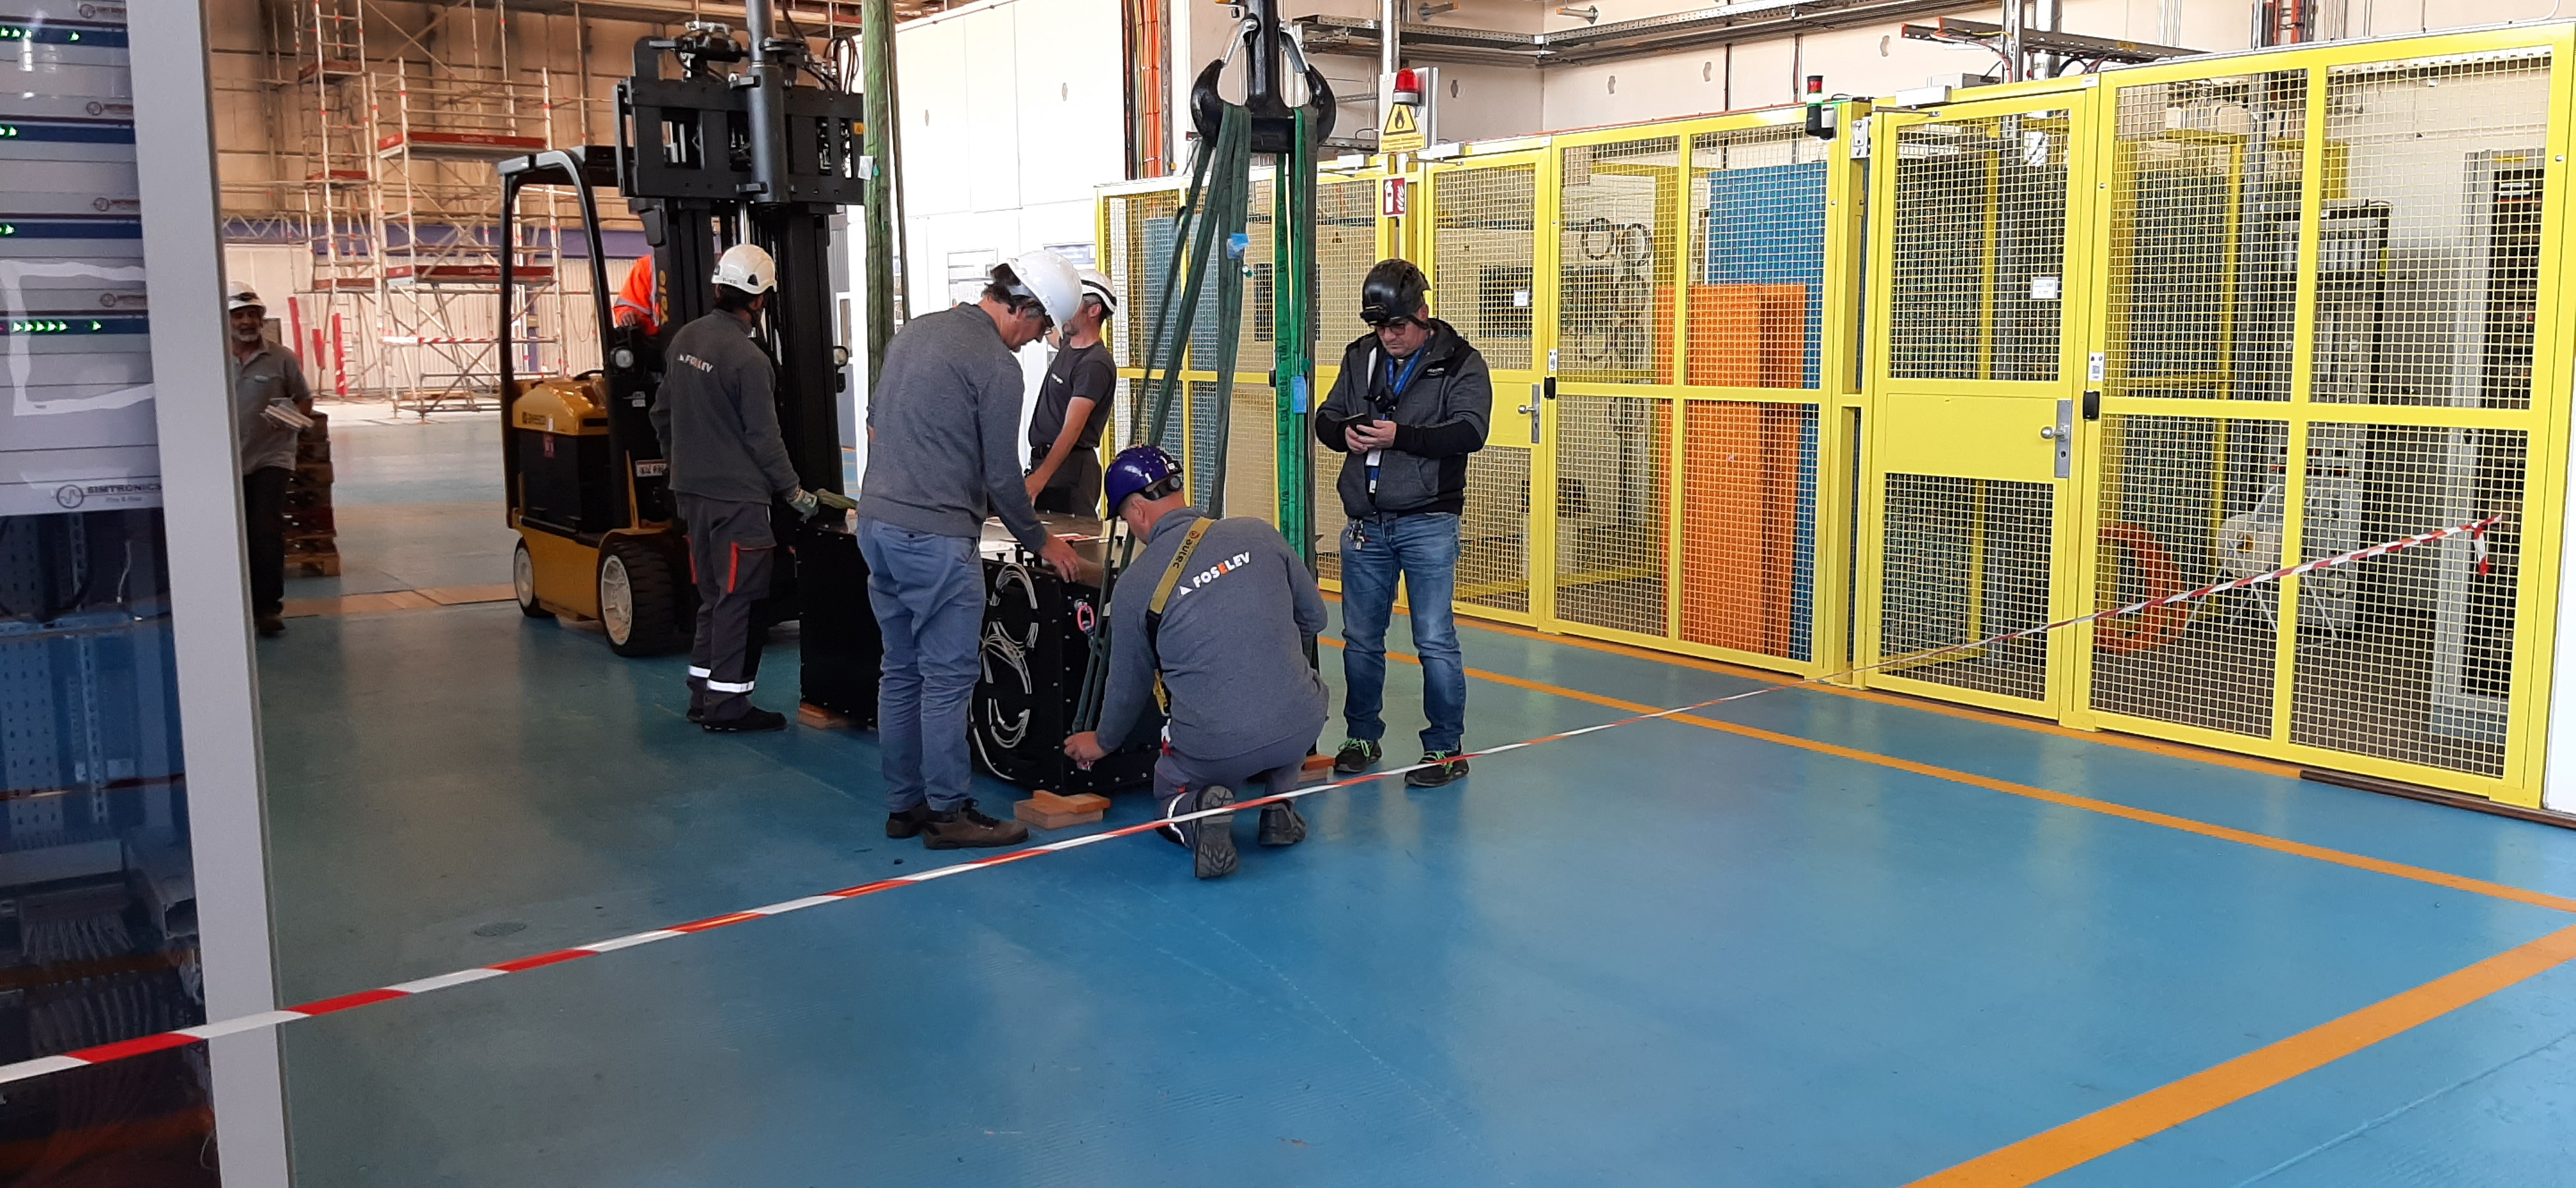
\includegraphics[width = 1.0\textwidth]{Plots/TORCH_transport_0.jpg}
    \caption{TORCH was transported horizontally}
  \end{figure}
\end{frame}

\begin{frame}{Week 2: TORCH arrives the zone}
  \begin{figure}
    \centering
    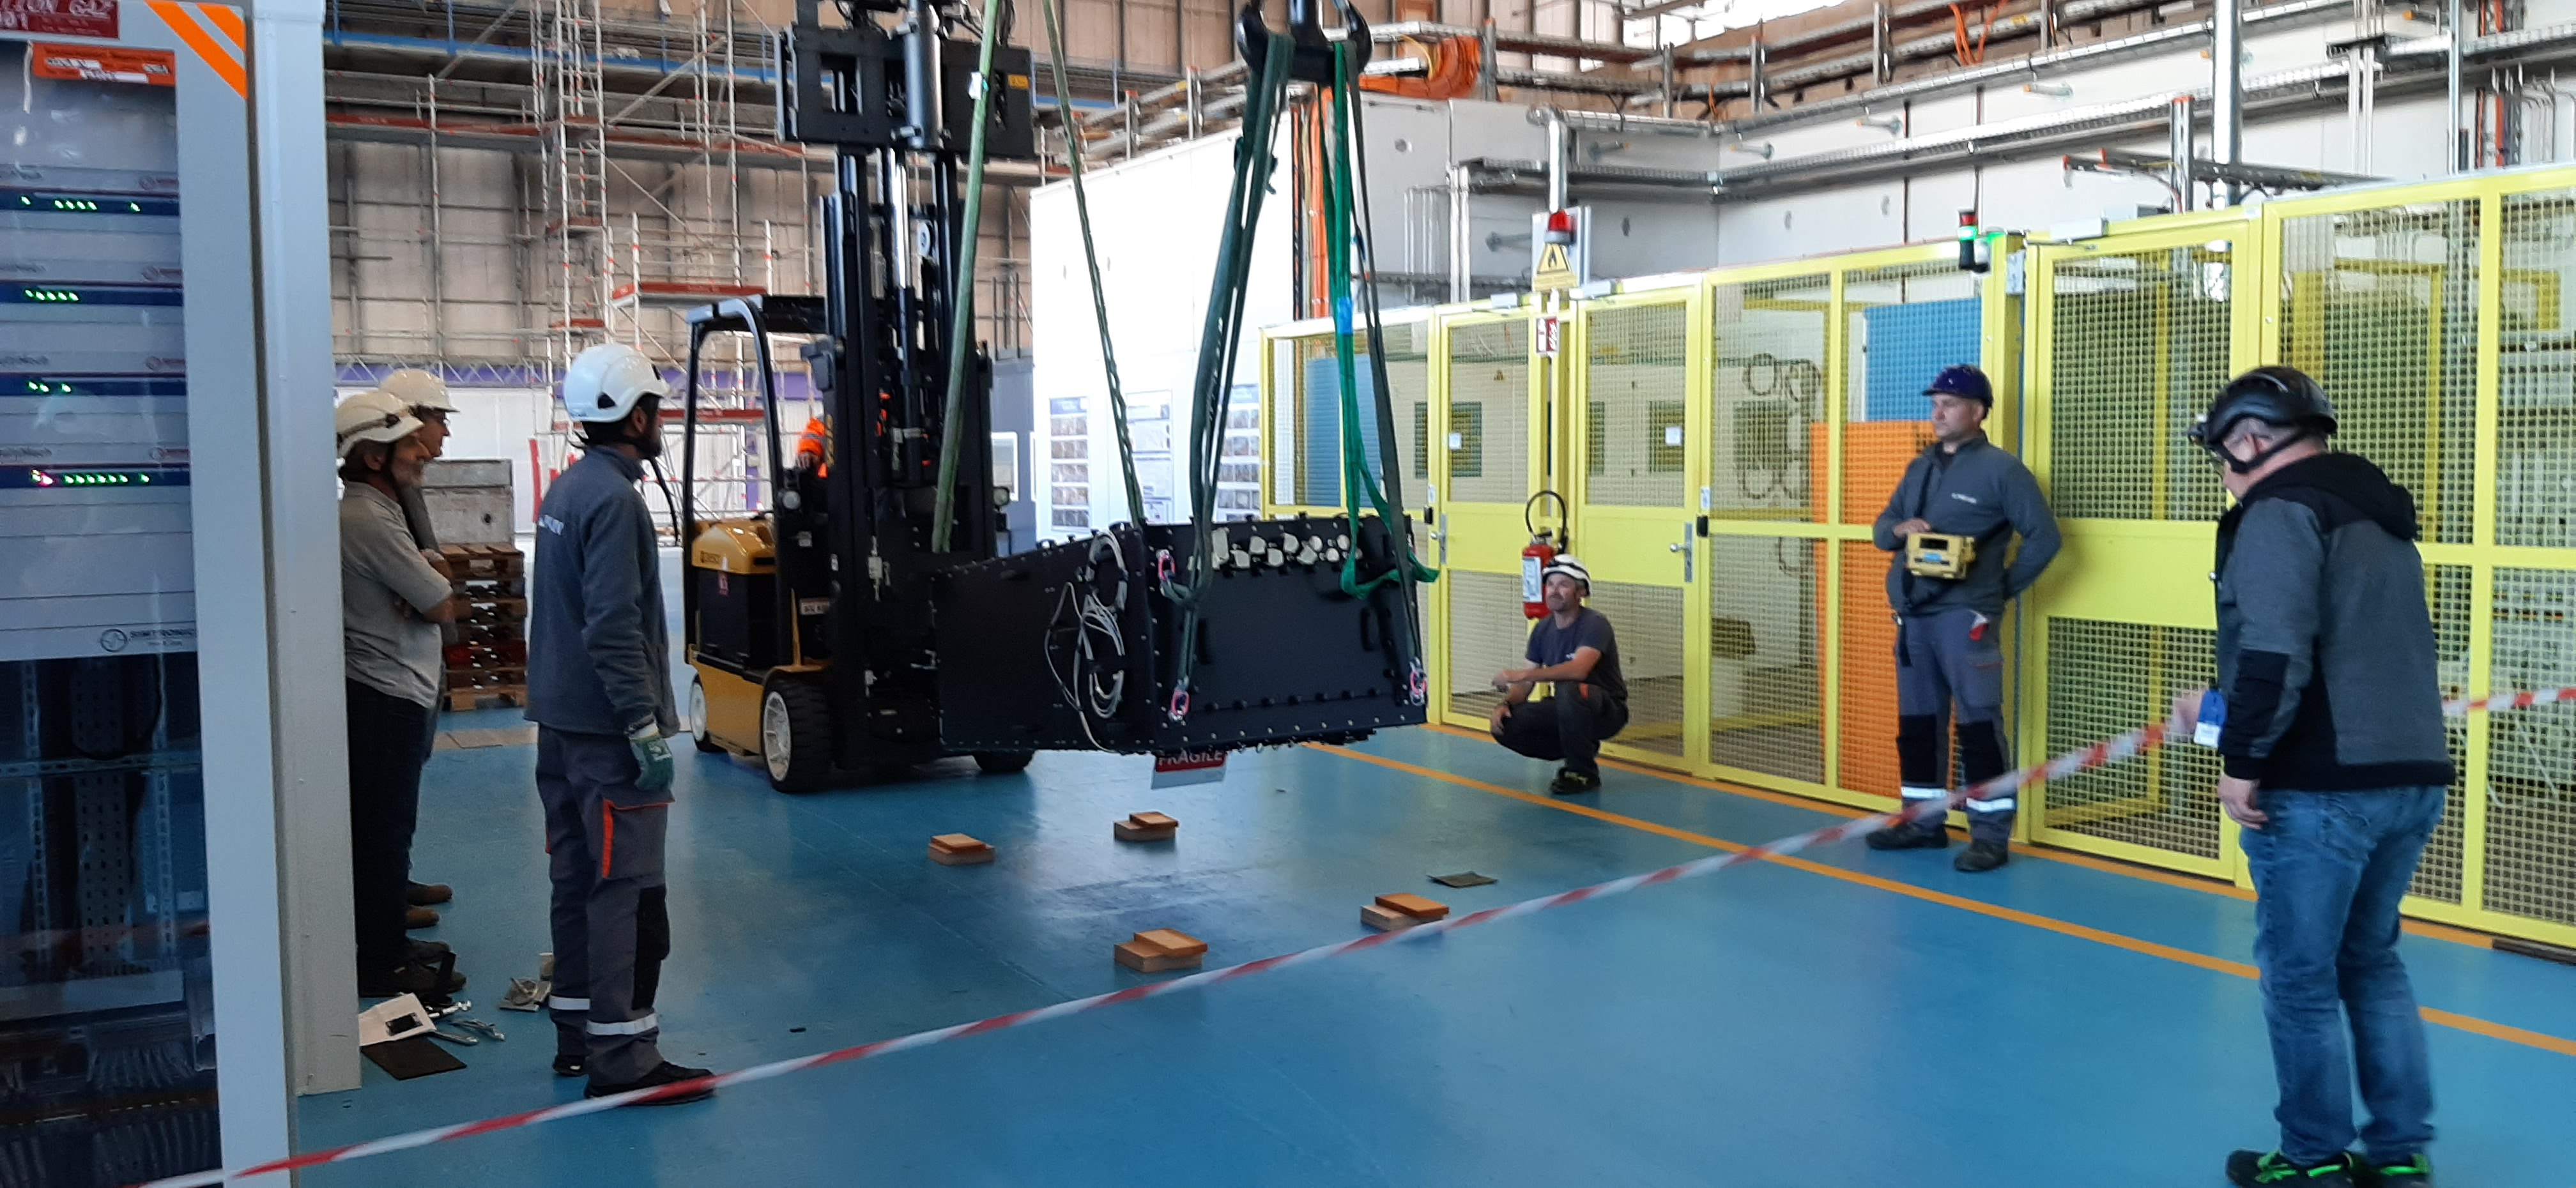
\includegraphics[width = 1.0\textwidth]{Plots/TORCH_transport_1.jpg}
    \caption{A crane and a forklift turns TORCH vertically}
  \end{figure}
\end{frame}

\begin{frame}{Week 2: TORCH arrives the zone}
  \begin{figure}
    \centering
    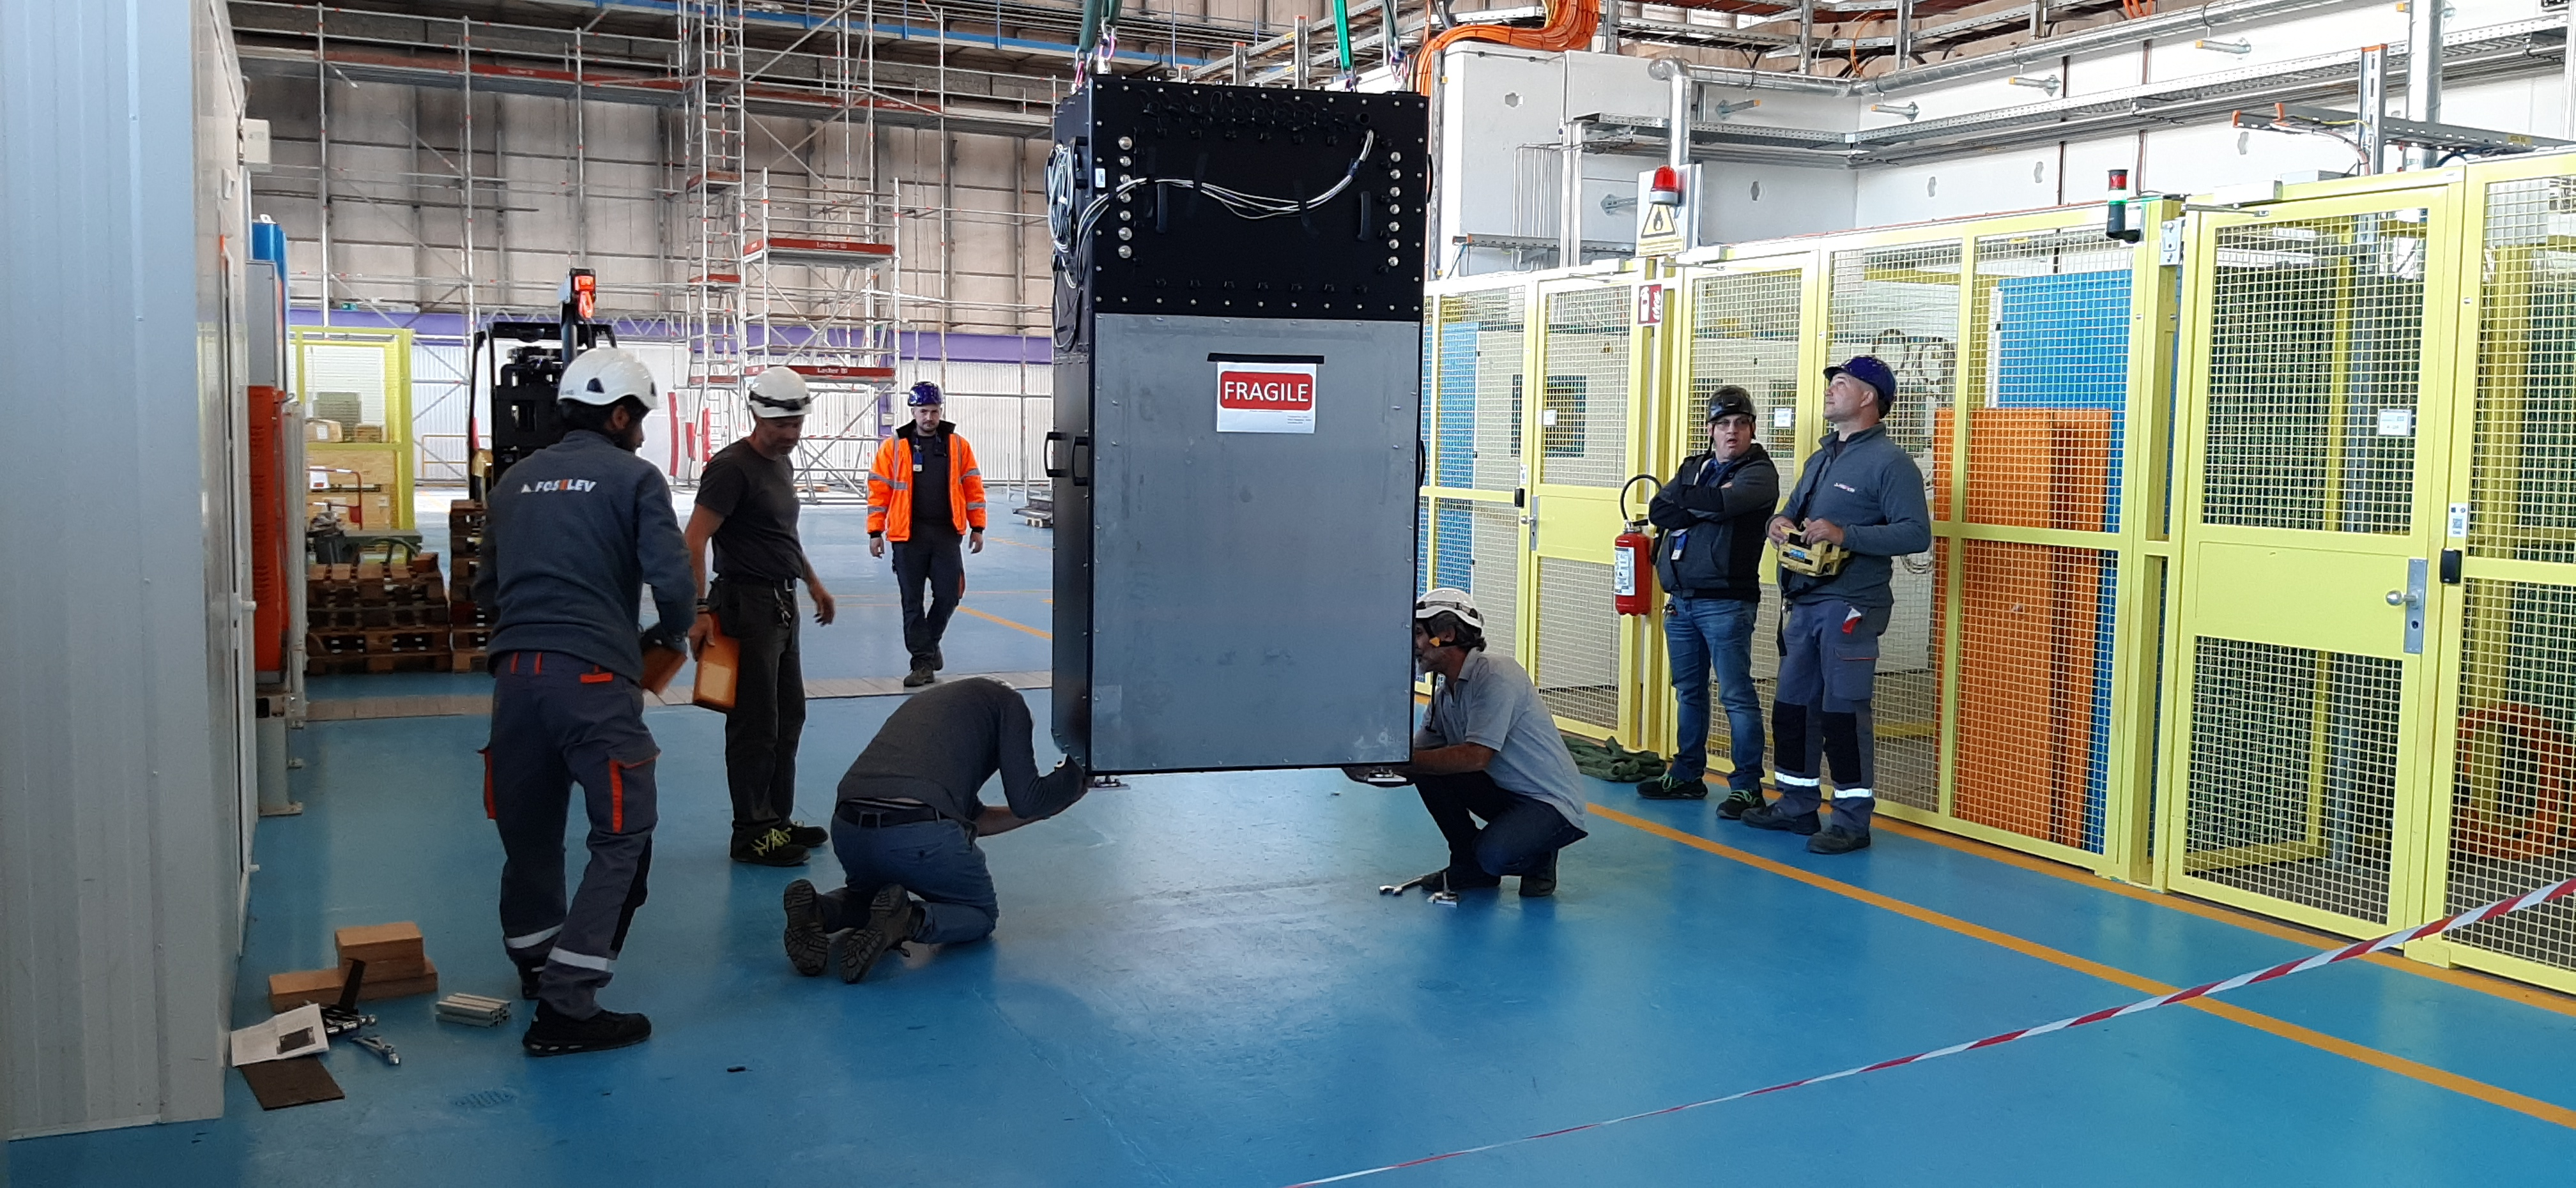
\includegraphics[width = 1.0\textwidth]{Plots/TORCH_transport_2.jpg}
    \caption{TORCH is ready to be lifted into the zone}
  \end{figure}
\end{frame}

\begin{frame}{Week 2: TORCH arrives the zone}
  \begin{figure}
    \centering
    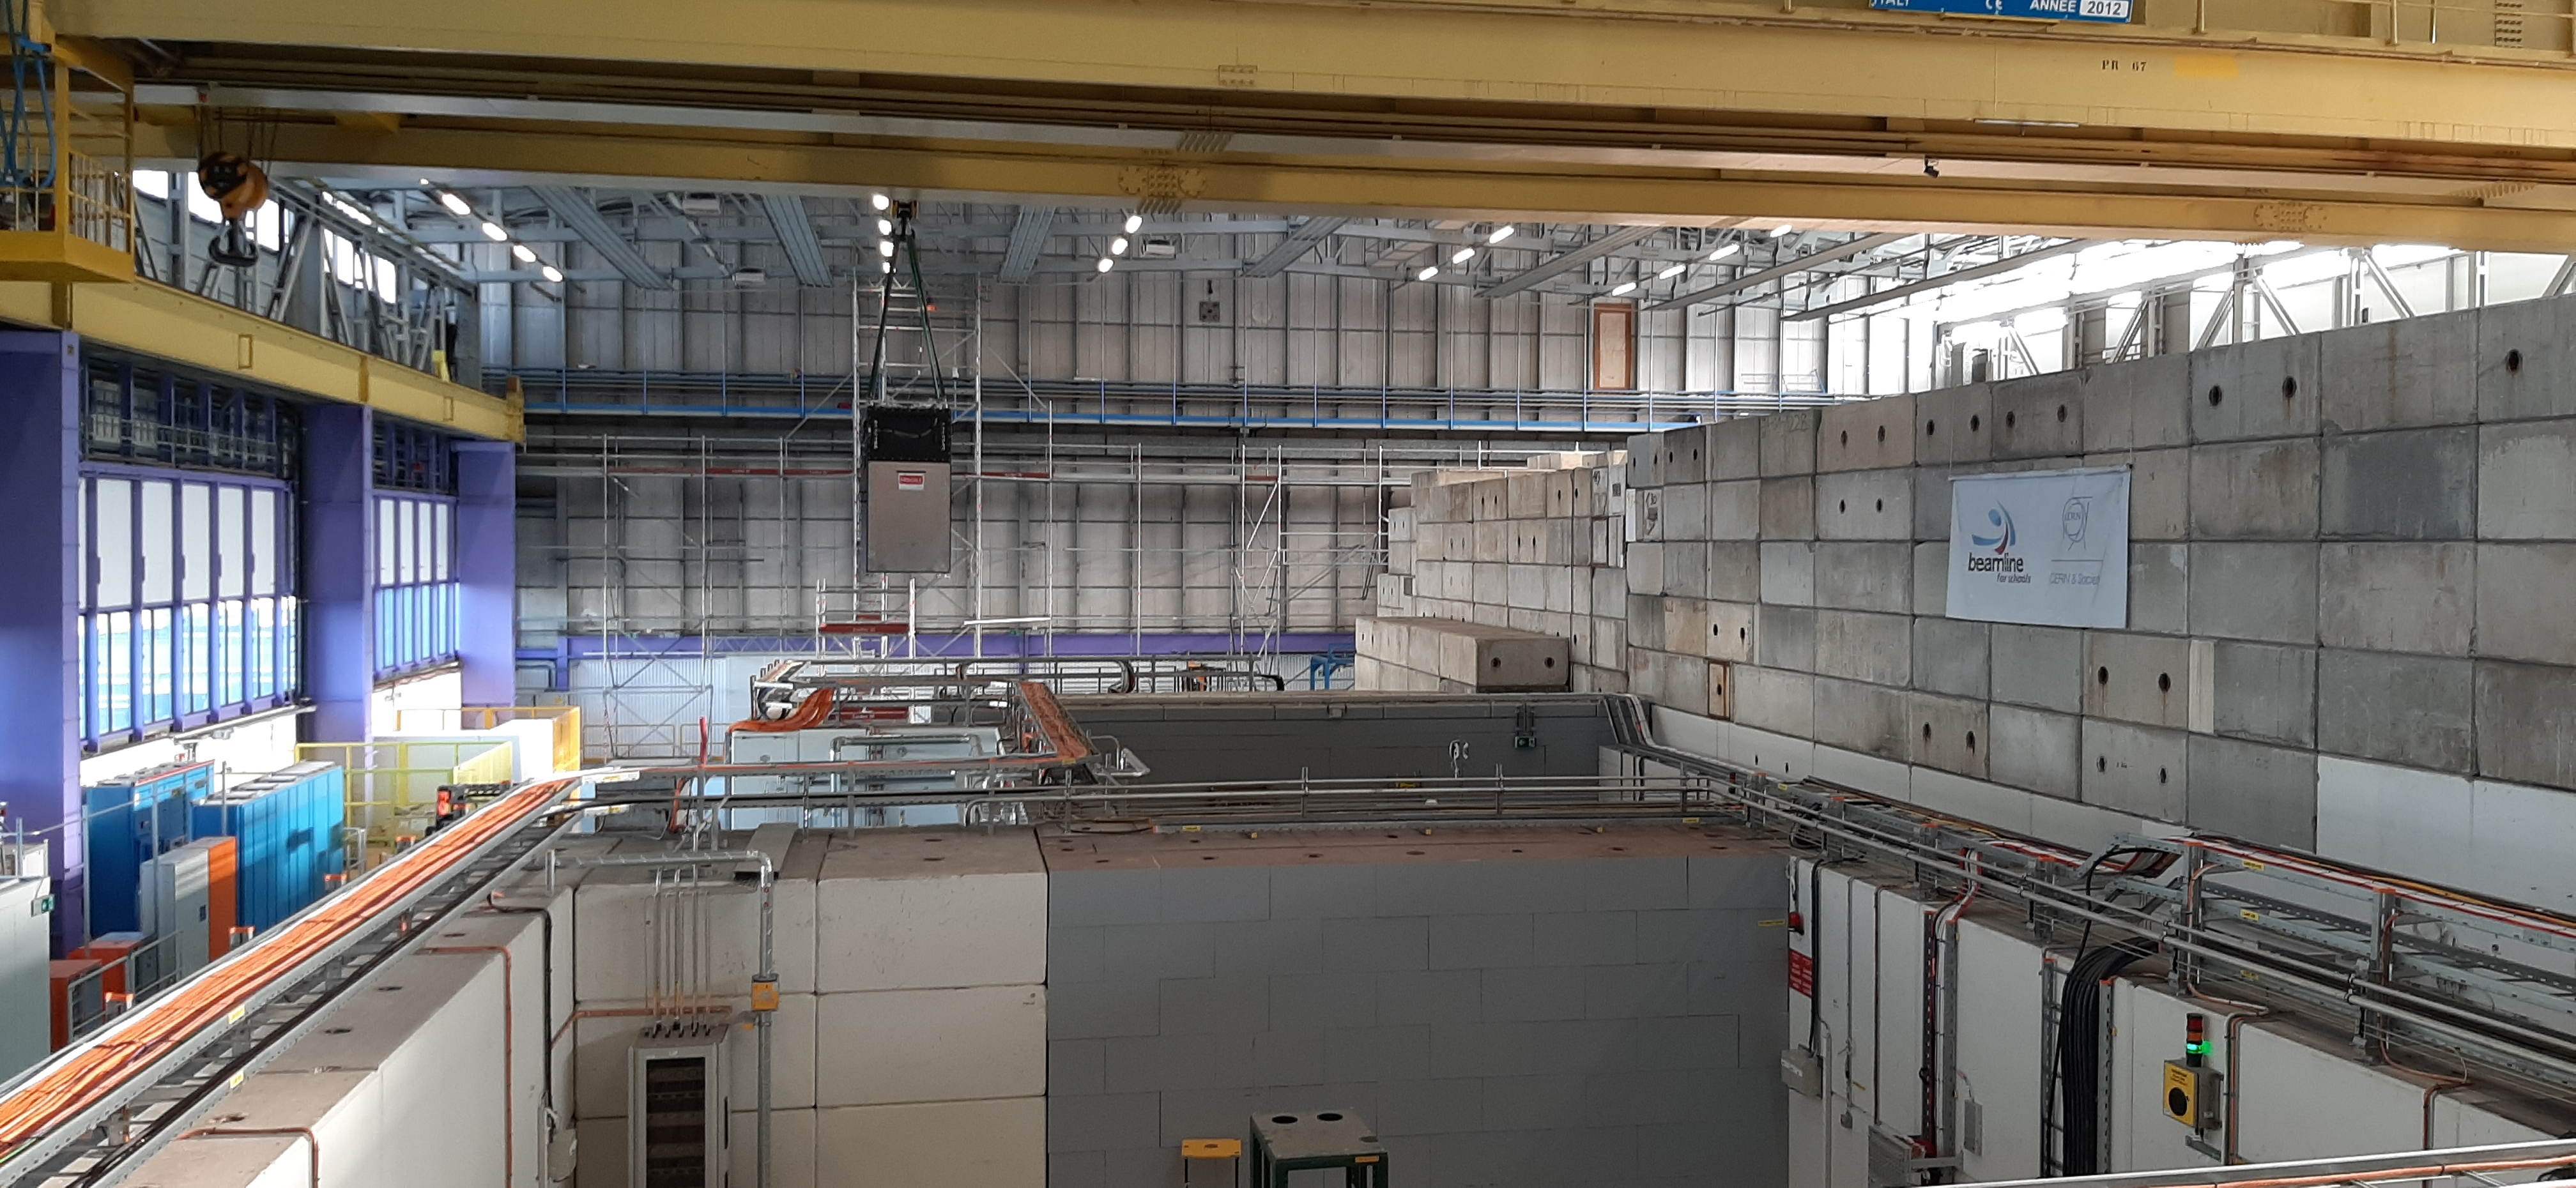
\includegraphics[width = 1.0\textwidth]{Plots/TORCH_transport_4.jpg}
    \caption{TORCH at its highest point}
  \end{figure}
\end{frame}

\begin{frame}{Week 2: TORCH arrives the zone}
  \begin{figure}
    \centering
    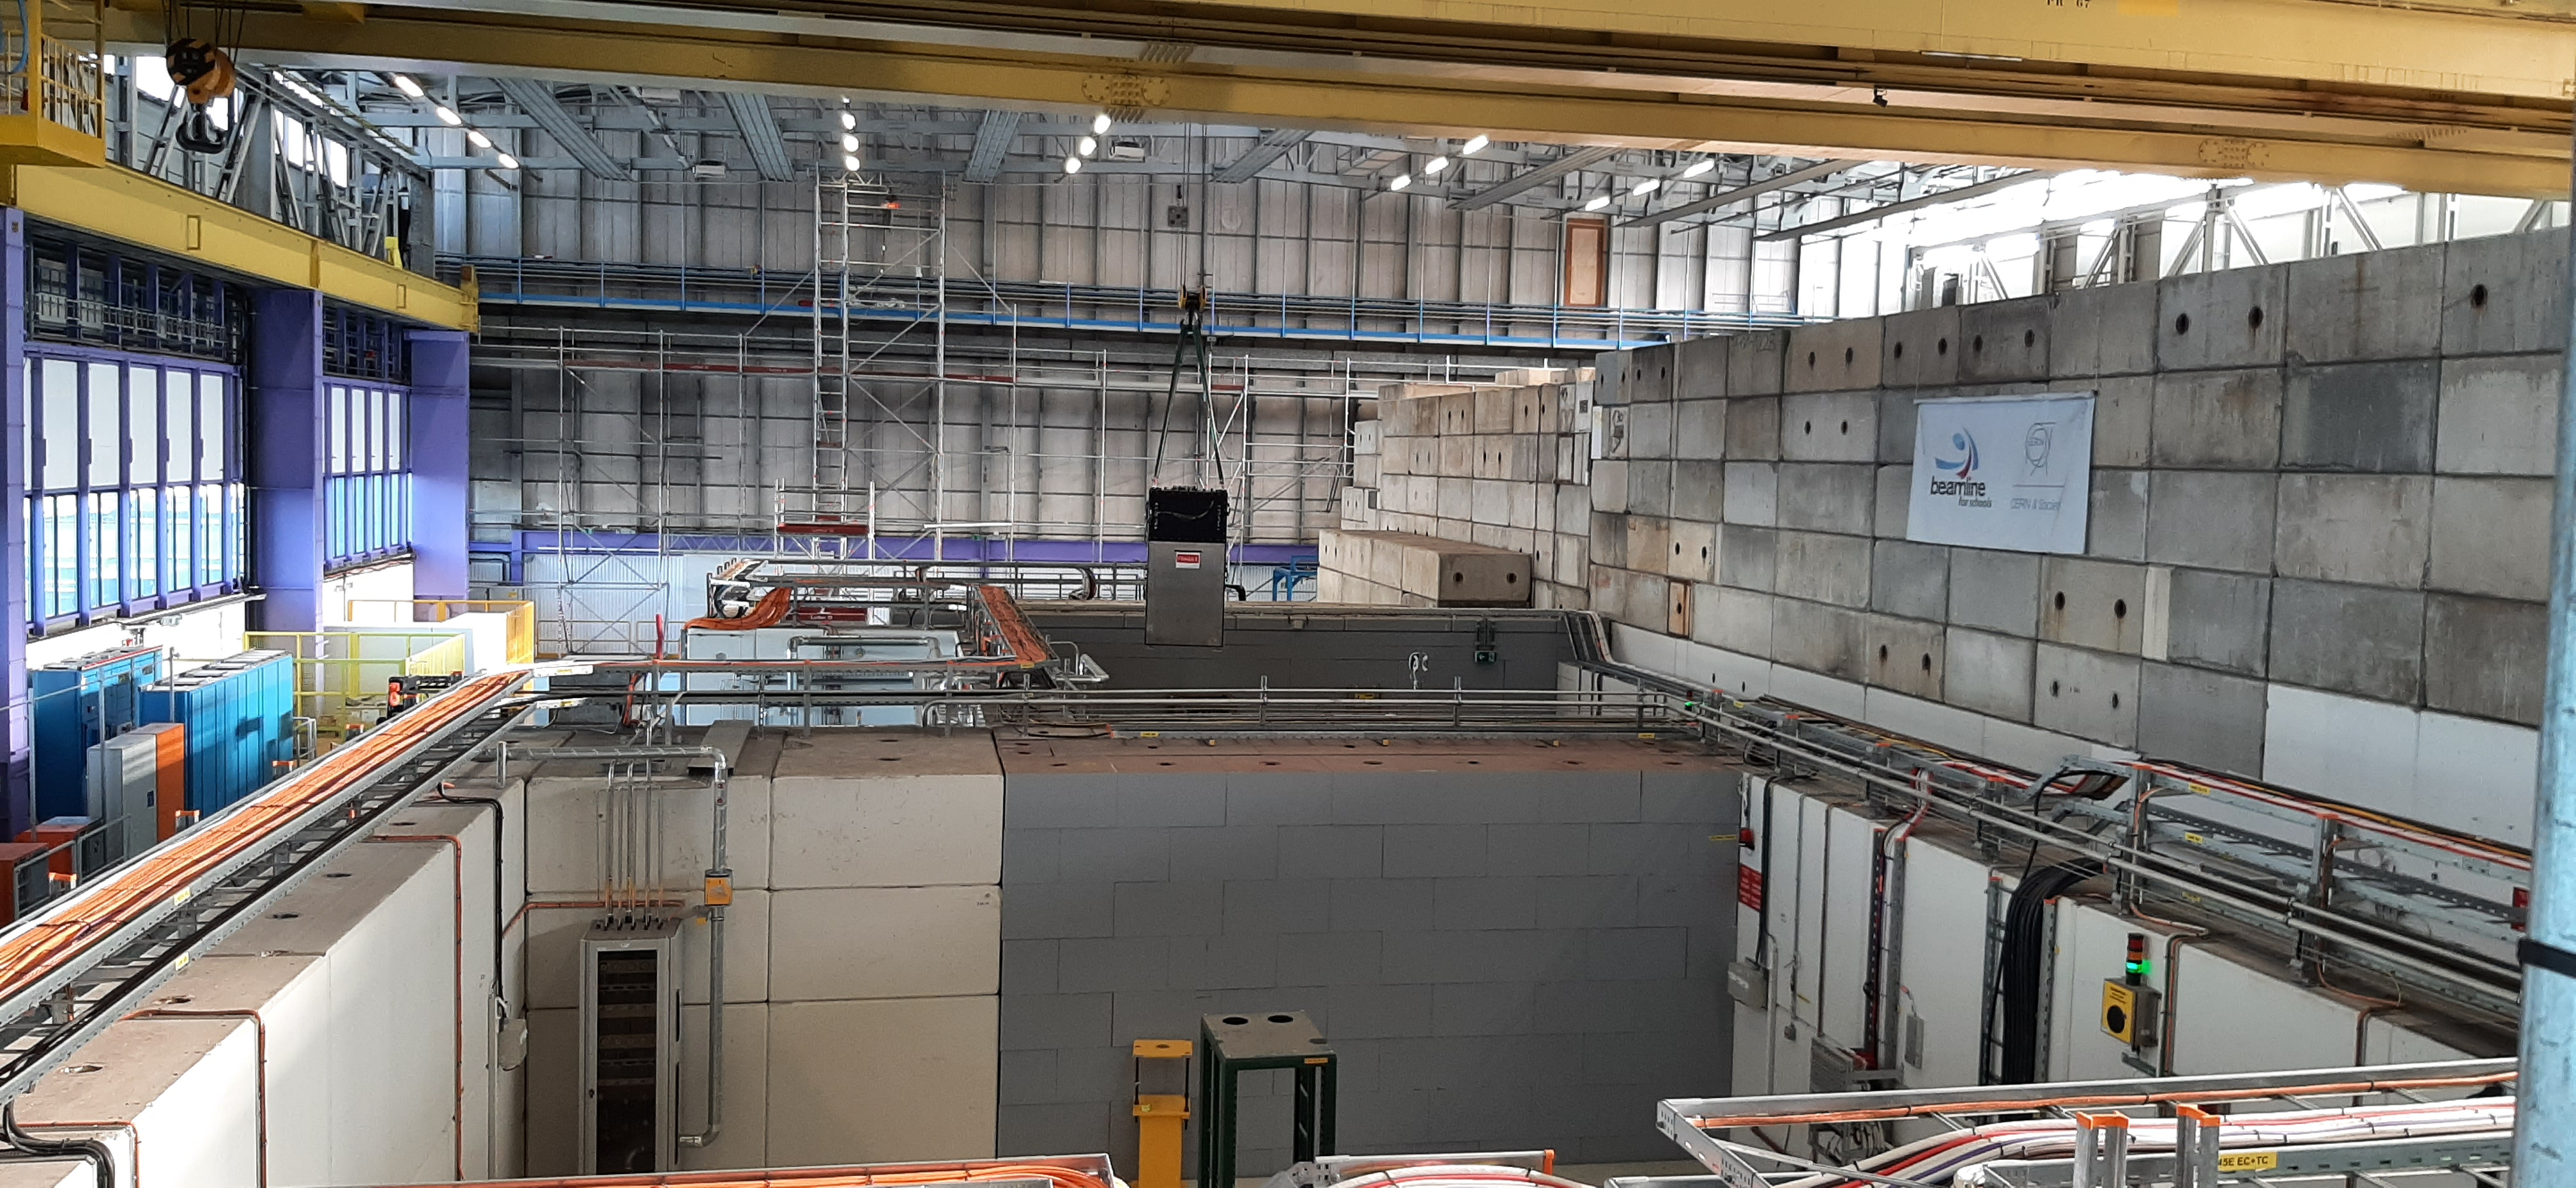
\includegraphics[width = 1.0\textwidth]{Plots/TORCH_transport_5.jpg}
    \caption{TORCH is then lowered into the zone}
  \end{figure}
\end{frame}

\begin{frame}{Week 2: TORCH arrives the zone}
  \begin{figure}
    \centering
    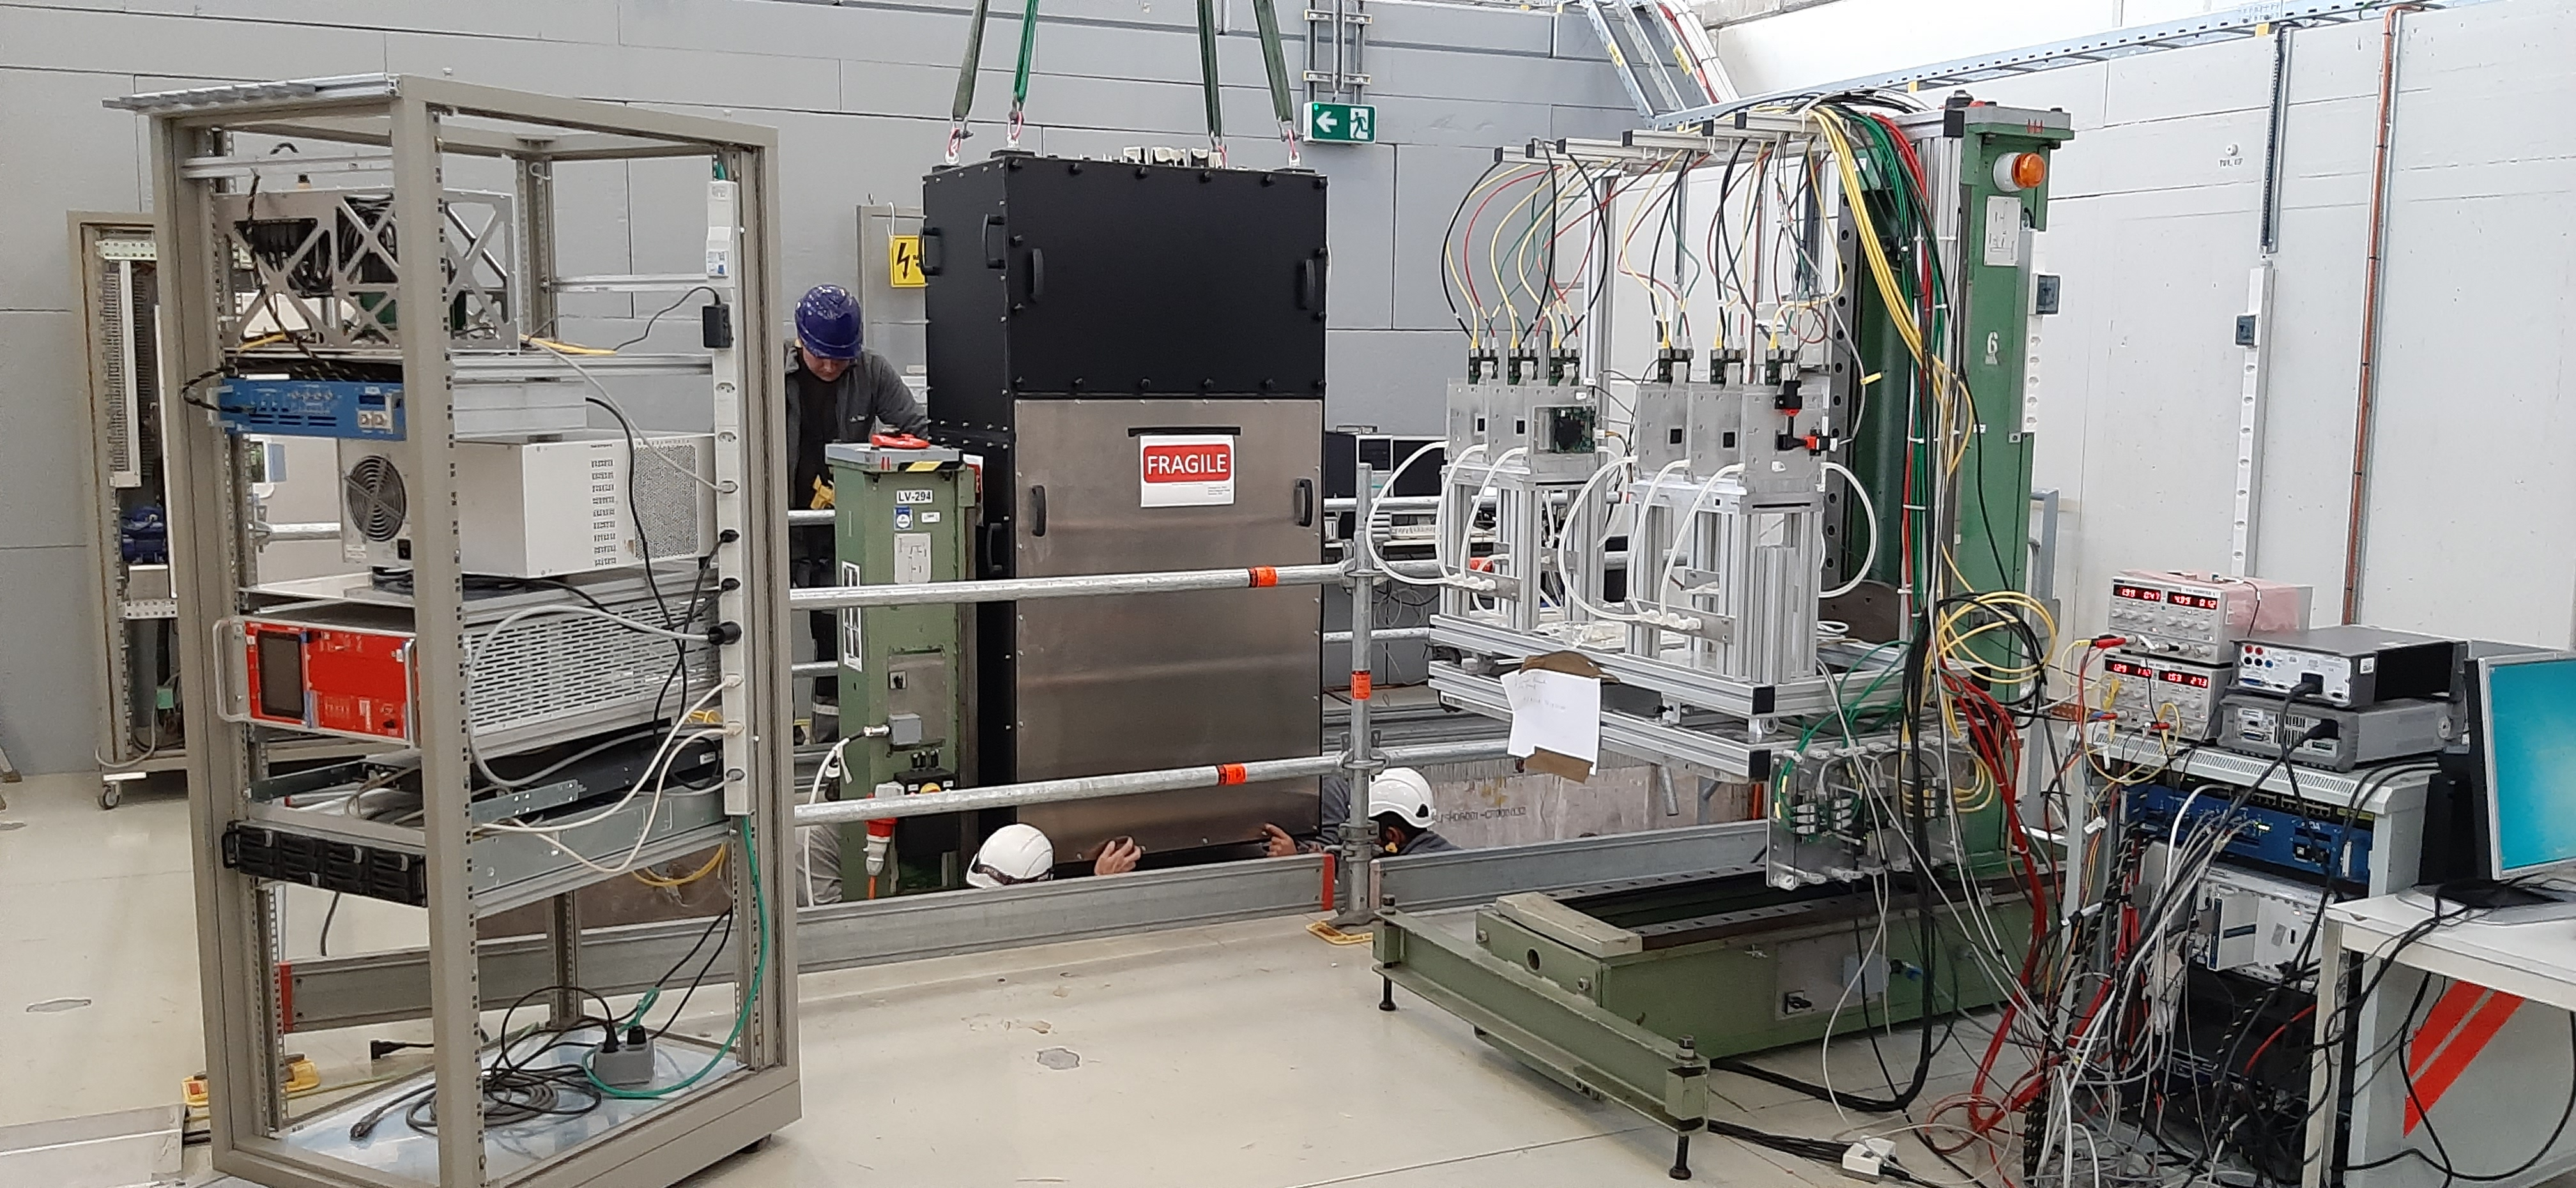
\includegraphics[width = 1.0\textwidth]{Plots/TORCH_transport_3.jpg}
    \caption{TORCH is safely on the DESY table}
  \end{figure}
\end{frame}

\begin{frame}{Week 2: TORCH arrives the zone}
  \begin{figure}
    \centering
    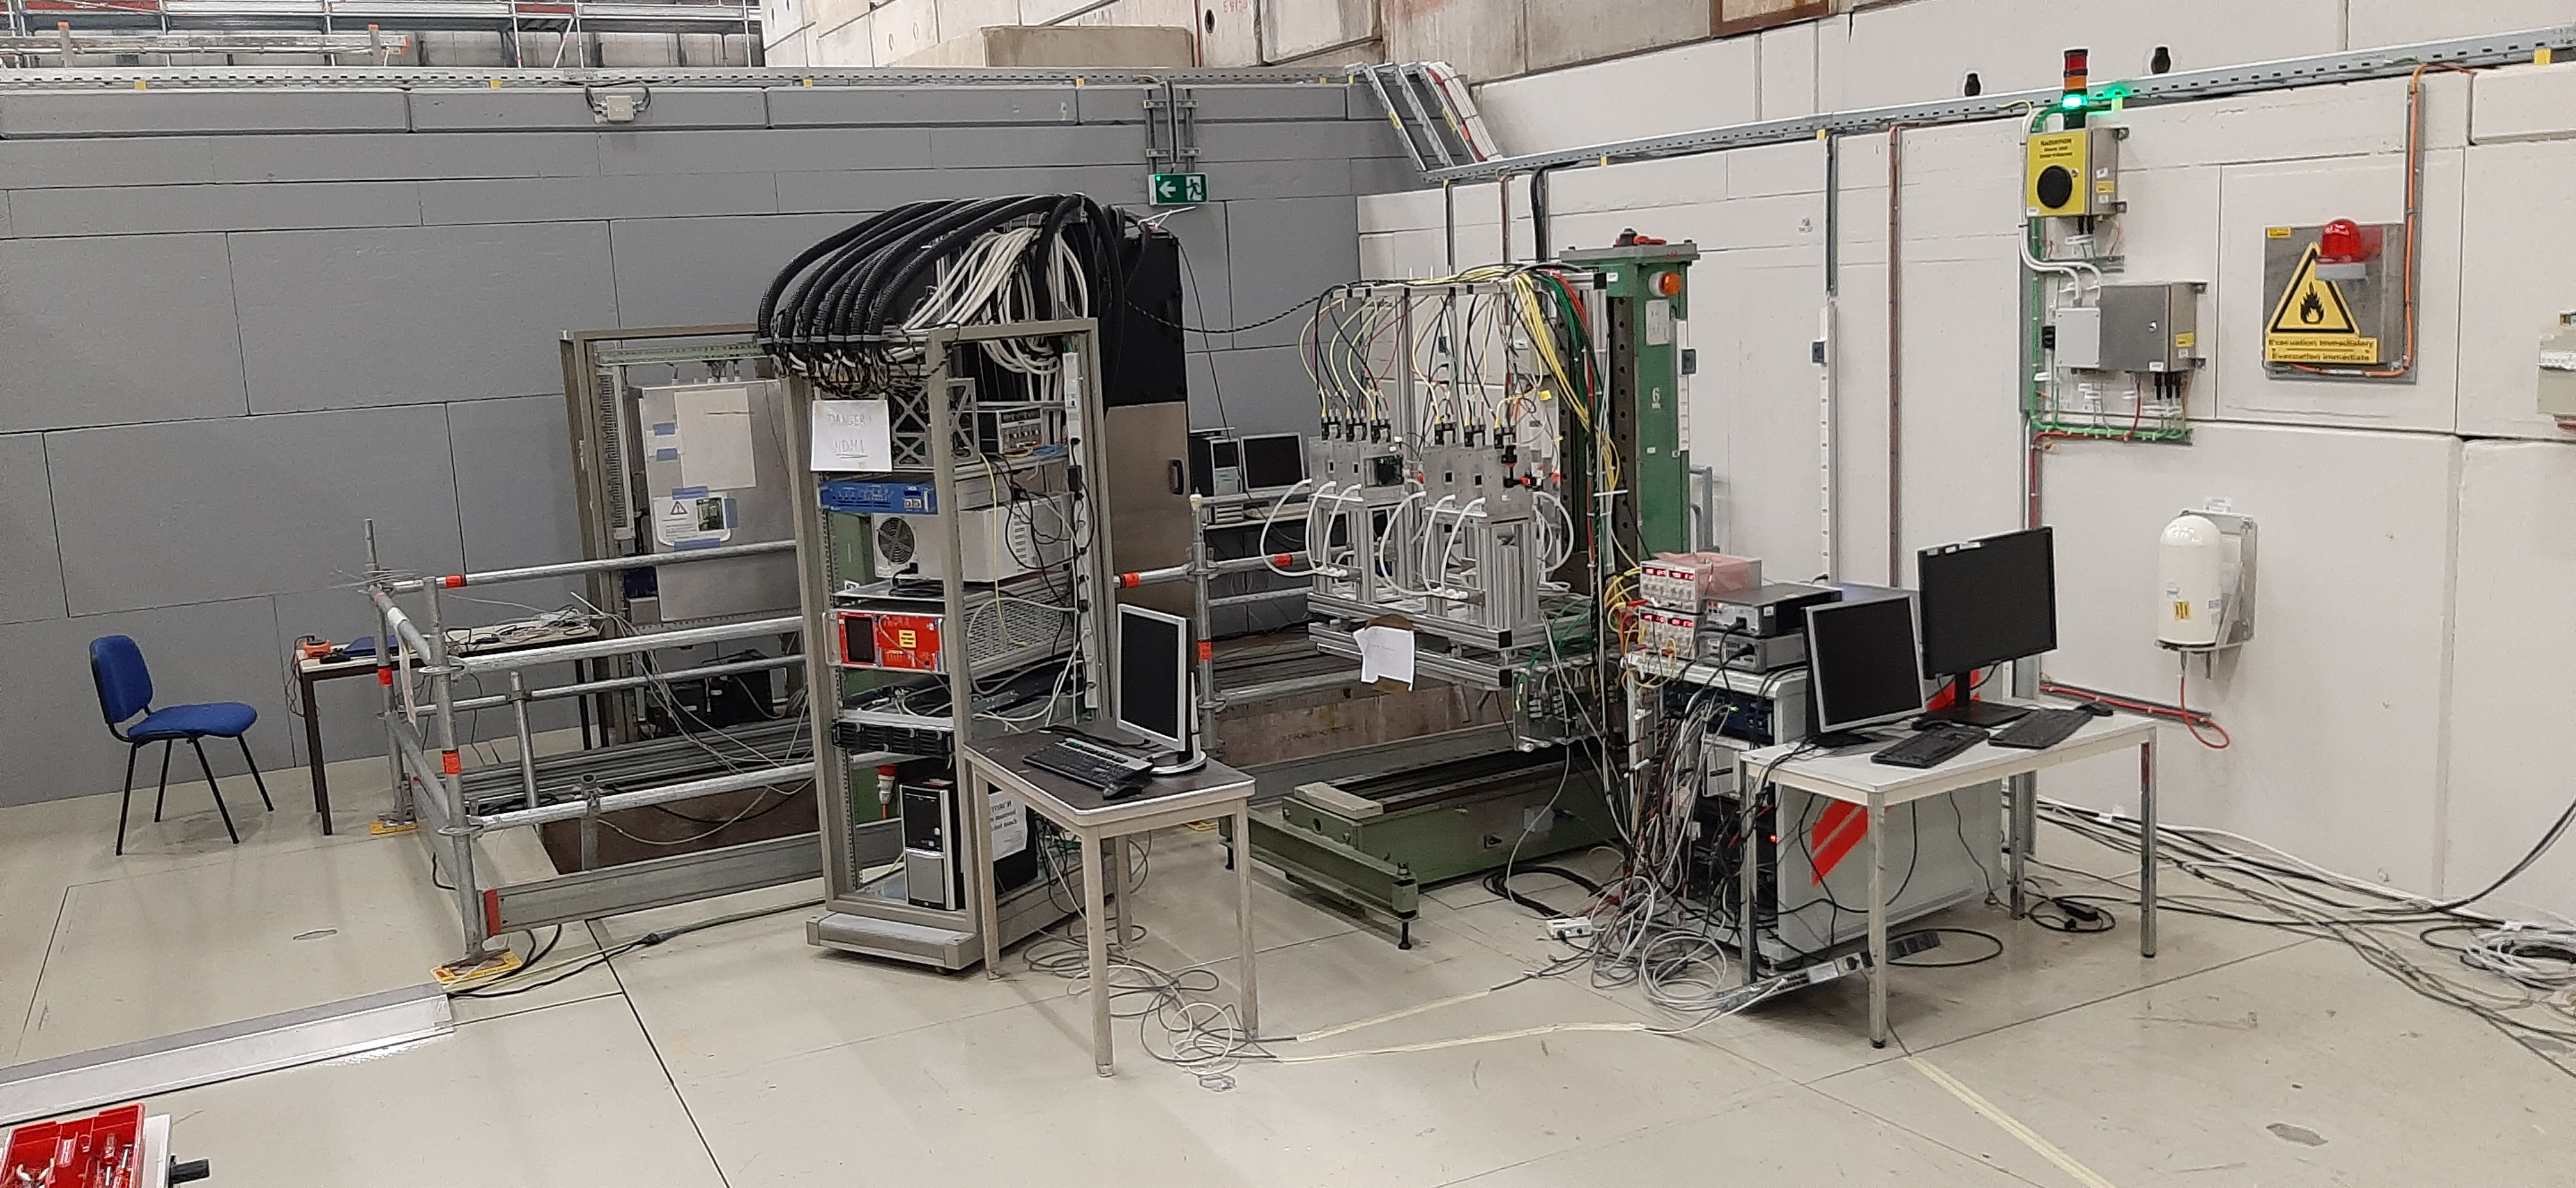
\includegraphics[width = 1.0\textwidth]{Plots/TelescopeTORCHoverview.jpg}
    \caption{TORCH and the beam telescope, with full cabling and cooling}
  \end{figure}
\end{frame}

\begin{frame}{Week 2: TORCH arrives the zone}
  \begin{figure}
    \centering
    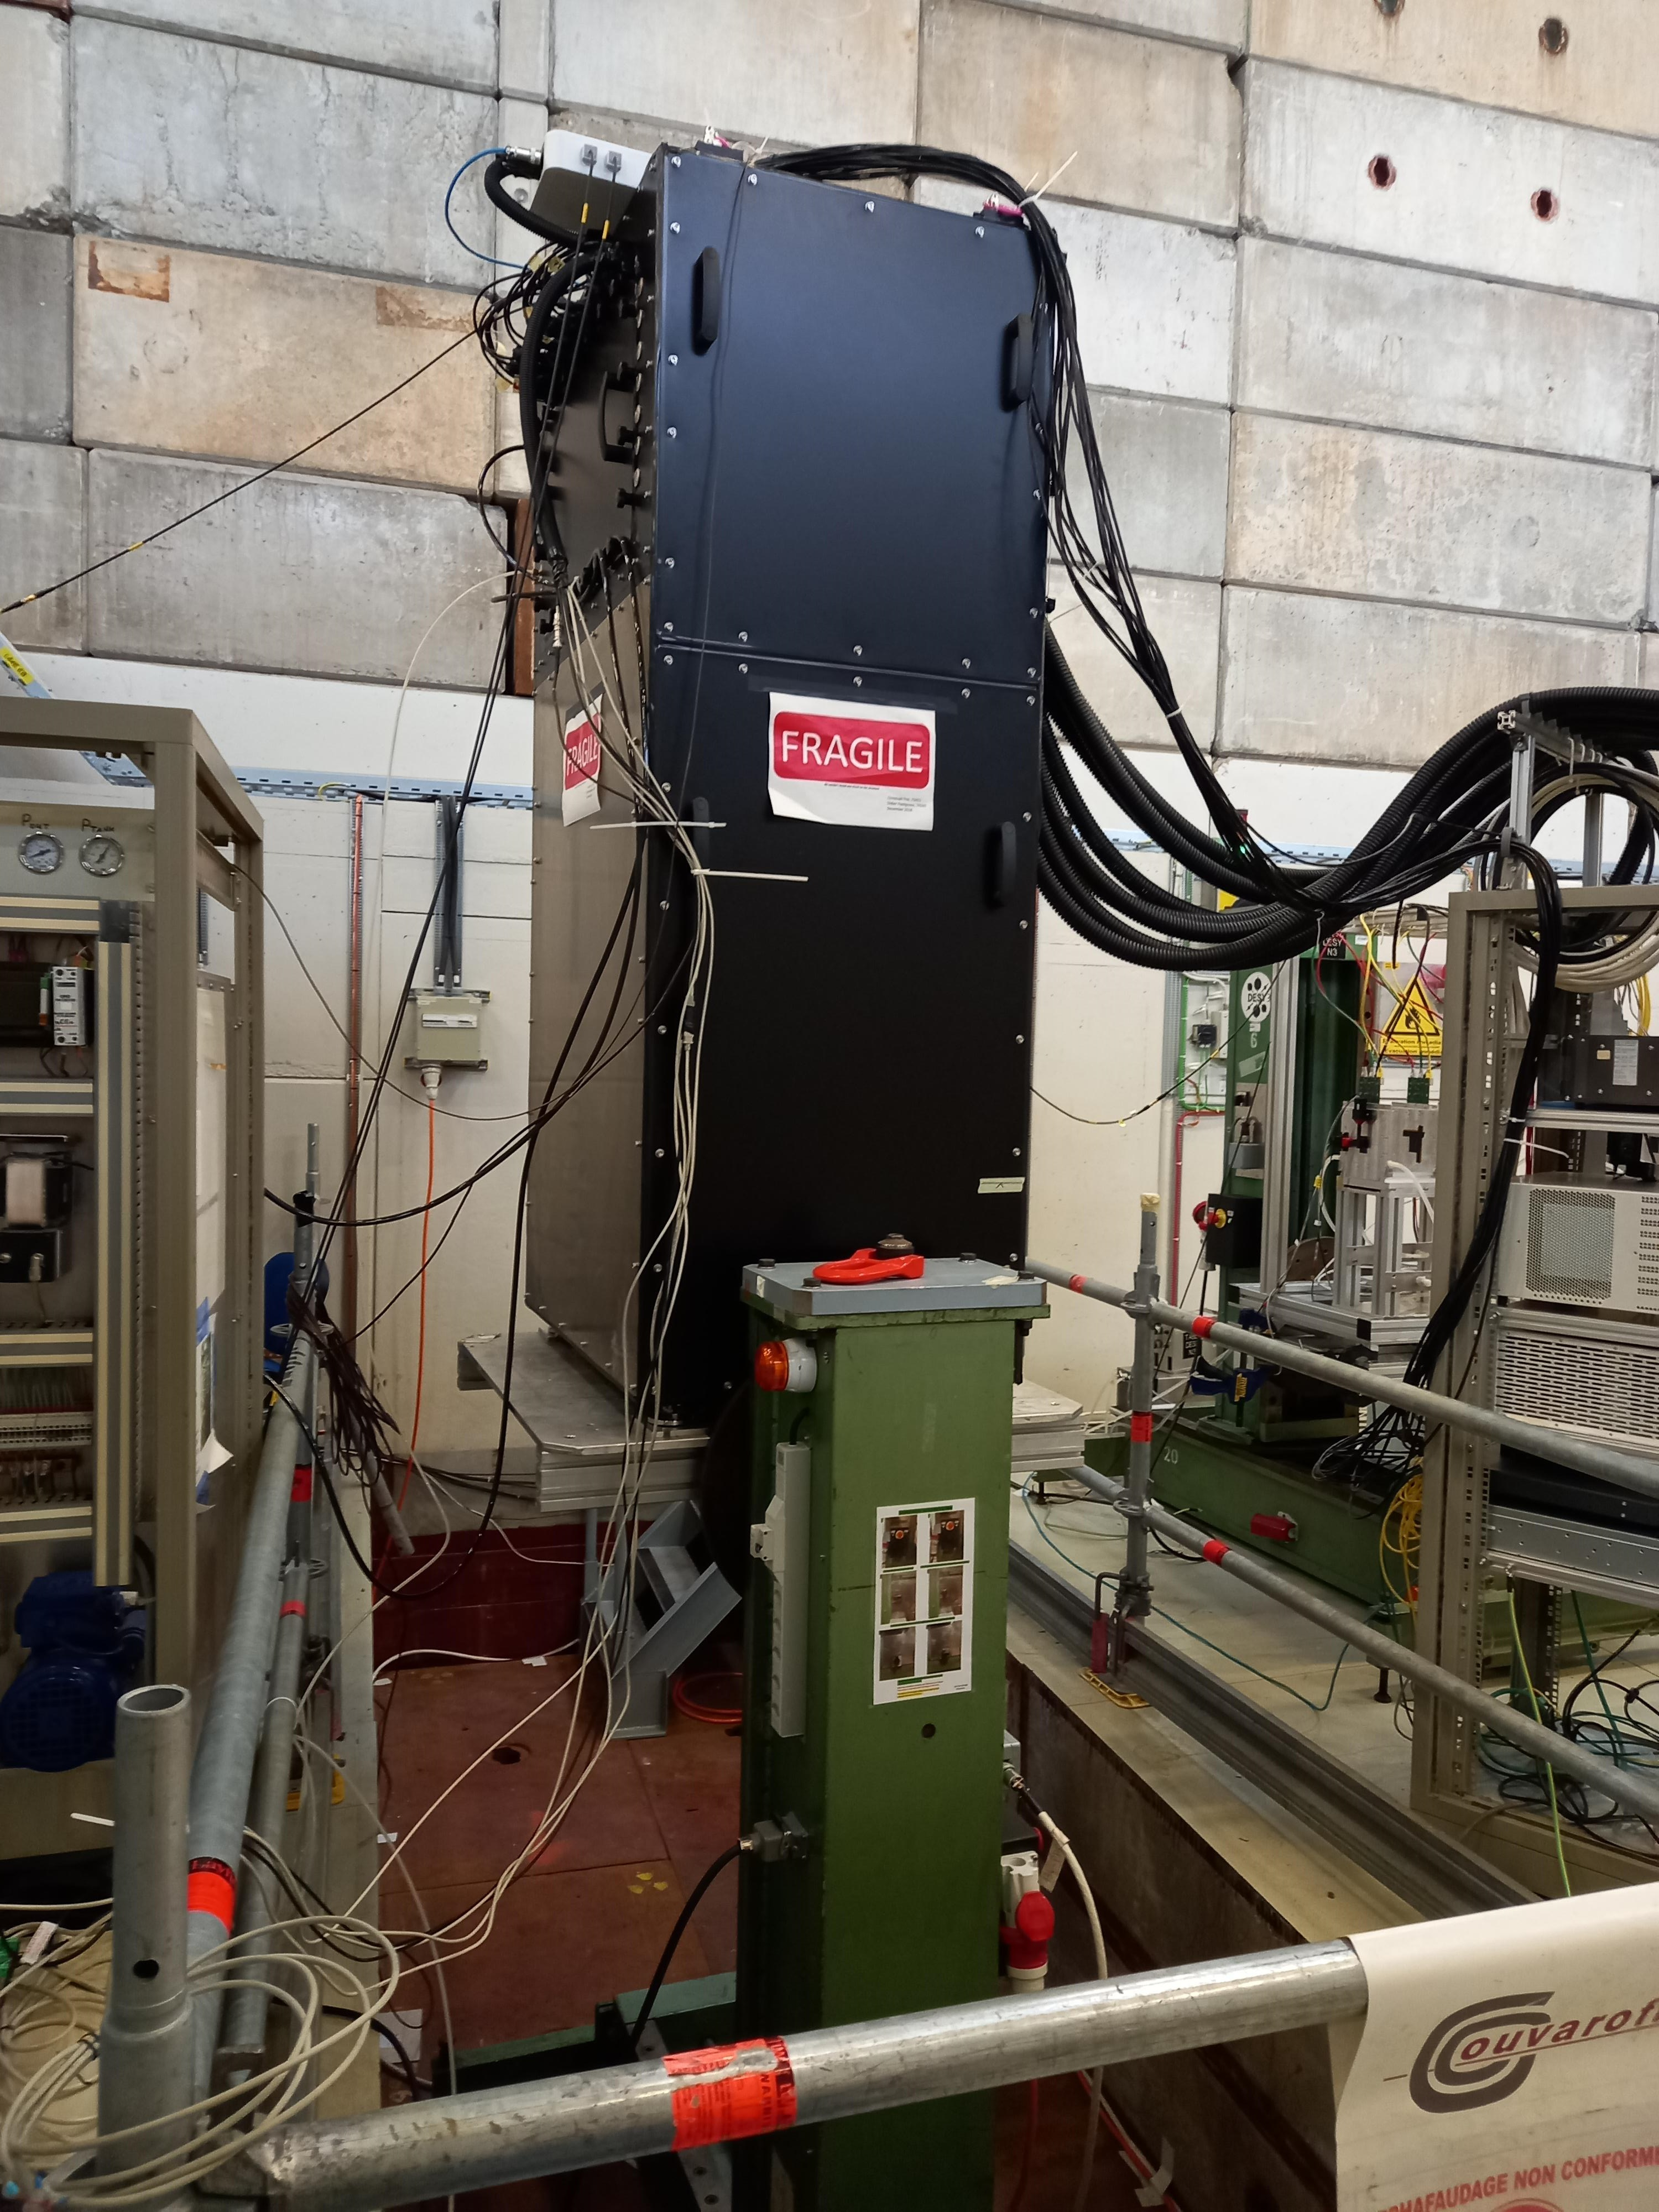
\includegraphics[width = 0.45\textwidth]{Plots/DESY_table.jpg}
    \caption{DESY table at its highest setting ($\SI{1}{\meter}$)}
  \end{figure}
\end{frame}

\begin{frame}{Summary and next steps}
  \begin{itemize}
    \setlength\itemsep{1.0em}
    \item{BESIII measurement of $c_i$ and $s_i$ is in the early stages}
    \begin{itemize}
      \item{Selection will be almost identical with the recent $F_+$ measurement}
      \item{Initial toy studies show that $c_i$ fits work}
      \item{Next steps:}
      \begin{enumerate}
        \item{Properly calculate bin efficiency/migration by training individual reweighters for each phase space bin}
        \item{Add selection of partially reconstructed $D\to KK\pi\pi$ vs CP tags}
        \item{Add the remaining $7$ CP tags and $K_{S, L}\pi\pi$ tags}
        \item{Aim to start charm WG review by end of TT23}
      \end{enumerate}
    \end{itemize}
    \item{TORCH testbeam done and PID studies will start soon}
    \begin{itemize}
      \item{I was involved with setting up trigger and time reference stations}
      \item{Next steps:}
      \begin{enumerate}
        \item{Initial studies and cross checks of November 2022 testbeam data}
        \item{Long term aim is to demonstrate PID separation power directly}
      \end{enumerate}
    \end{itemize}
  \end{itemize}
  \begin{center}
    \huge Thank you for listening!
  \end{center}
\end{frame}

\end{document}
